%UCSD Master's Thesis - Kevin Chau, Biology 2019
% ----------------------------------------------------------------------
% BUILDING:
%
%   This document was built with pdflatex
%
% ----------------------------------------------------------------------
% More control of the formatting of your thesis can be achieved through
% modifications of the included LaTeX class files:
%
%   * ucsd.cls    -- Class file
%   * uct10.clo   -- Configuration files for font sizes 10pt, 11pt, 12pt
%     uct11.clo                            
%     uct12.clo
%
% ----------------------------------------------------------------------



% Setup the documentclass 
% default options: 12pt, oneside, final
%
% fonts: 10pt, 11pt, 12pt -- are valid for UCSD dissertations.
% sides: oneside, twoside -- note that two-sided theses are not accepted 
%                            by OGS.
% mode: draft, final      -- draft mode switches to single spacing, 
%                            removes hyperlinks, and places a black box
%                            at every overfull hbox (check these before
%                            submission).
% chapterheads            -- Include this if you want your chapters to read:
%                              Chapter 1
%                              Title of Chapter
%
%                            instead of
%                              1 Title of Chapter
\documentclass[12pt,chapterheads,final]{ucsd}


%% GRAPHICX - This is the standard package for 
%    including graphics for latex/pdflatex.
\usepackage{scrextend}
\usepackage{pslatex}
\usepackage{graphicx}

%% CAPTION
% This overrides some of the ugliness in ucsd.cls and
% allows the text to be double-spaced while letting figures,
% tables, and footnotes to be single-spaced--all OGS requirements.
% NOTE: Must appear after graphics and ams math
\makeatletter
\gdef\@ptsize{2}% 12pt documents
\let\@currsize\normalsize
\makeatother
\usepackage{setspace}
\doublespace
\usepackage[font=small, width=0.9\textwidth]{caption}

%% CITATIONS
% Sets citation format
% and fixes up citations madness
\usepackage{microtype}  % avoids citations that hang into the margin


%% FOOTNOTE-MAGIC
% Enables footnotes in tables, re-referencing the same footnote multiple times.
\usepackage{footnote}
\makesavenoteenv{tabular}
\makesavenoteenv{table}


%% TABLE FORMATTING MADNESS
% Enable all sorts of fun table tricks
\usepackage{rotating}  % Enables the sideways environment (NCPW)
\usepackage{array}  % Enables "m" tabular environment http://ctan.org/pkg/array
\usepackage{booktabs}  % Enables \toprule  http://ctan.org/pkg/array

\usepackage{chngcntr}
\counterwithout{figure}{chapter}

\begin{document}

%% FRONT MATTER
%
%  All of the front matter.
%  This includes the title, degree, dedication, vita, abstract, etc..
%  Modify the file template_frontmatter.tex to change these pages.
%
%UCSD Master's Thesis - Kevin Chau, Biology 2019
% ----------------------------------------------------------------------
%

\title{Isoform transcriptome of developing brain provides new insights into autism risk variants}

\author{Kevin Khai Chau}
\degreeyear{2019}

\degreetitle{Master of Science}

\field{Biology}

\chair{Lilia M. Iakoucheva}
\cochair{Scott Rifkin}

%  The rest of the committee members  must be alphabetized by last name.
\othermembers{
Barry Grant\\
}
\numberofmembers{3} % |chair| + |cochair| + |othermembers|


%% START THE FRONTMATTER
\begin{frontmatter}

%% TITLE PAGES
\makefrontmatter

%% SETUP THE TABLE OF CONTENTS
\tableofcontents
\listoffigures
\listofsuppfigures
\listoftables

%% ACKNOWLEDGEMENTS
\begin{acknowledgements}
I would like to acknowledge Professor Lilia M. Iakoucheva for her support as the chair of my committee. \par
I would also like to thank my post-doctoral mentor Dr. Pan Zhang for his guidance throughout this project, as well as Dr. Patricia M. Losada, Dr. Akula Bala Pramod, Dr. Jorge Urresti, and Dr. Megha Amar for all of their support. \par
This thesis, in full, is currently being prepared for submission for publication of the material. Chau, Kevin K.; Zhang, Pan; Urresti, Jorge; Amar, Megha; Pramod, Akula Bala; Corominas, Roser; Lin, Guan Ning; Iakoucheva, Lilia M. The thesis author was the primary investigator and author of this material. \par
\end{acknowledgements}


\begin{abstract}
Alternative splicing plays important role in brain development, however its global contribution to human neurodevelopmental diseases (NDD) has not been fully investigated. Here, we examined the relationship between splicing isoform expression and \textit{de novo} loss-of-function mutations implicated in autism. We constructed isoform transcriptome of the developing human brain, and observed better resolution and stronger signals at the isoform-level compared to the gene-level transcriptome. We identified differentially expressed isoforms and isoform co-expression modules enriched in autism loss-of-function mutations. These isoforms have higher prenatal expression, are enriched in microexons, and are co-expressed with a unique set of partners. We experimentally test the impact of splice site mutations in five NDD risk genes, including \textit{SCN2A}, \textit{DYRK1A} and \textit{BTRC}, and demonstrate exon skipping. Furthermore, our results suggest that the splice site mutation in \textit{BTRC} reduces its translational efficiency, likely impacting Wnt signaling through impaired degradation of $\beta$-catenin. We propose that functional effect of mutations associated with human diseases should be investigated at isoform- rather than gene-level resolution.

\end{abstract}


\end{frontmatter}


%% THESIS

% A common strategy here is to include files for each of the chapters. I.e.,
% Place the chapters is separate files: 
%   chapter1.tex, chapter2.tex
% Then use the commands:
%   \include{chapter1}
%   \include{chapter2}
%
% Of course, if you prefer, you can just start with
%   \chapter{My First Chapter Name}
% and start typing away. 

\chapter{Introduction}
More than 95\% of multi-exon human genes undergo alternative splicing (AS) and/or use alternative promoters to increase transcriptomic and proteomic diversity, with an estimated average of five to seven isoforms transcribed per gene \cite{Wang2008,Pan2008,Steijger2013}. Alternative splicing is highly specific, and expression of isoforms is often restricted to certain organs, tissues or cell types \cite{Trapnell2010,Barbosa-Morais2012,Sapkota2019,Shalek2013}. In addition, many isoforms are expressed only during specific developmental periods \cite{Kalsotra2011}. The developing human brain exhibits one of the highest frequencies of alternative splicing events \cite{Yeo2004,Calarco2011,Mele2015,Raj2015}. Many of the processes occurring during neural development are controlled by differentially expressed alternatively spliced isoforms \cite{Li2007,Kim2013,Grabowski2011}. Several recent studies, including one by us, began to investigate isoform-level transcriptome dysregulation in psychiatric diseases \cite{Parikshak2016,Gandal2018,Li2018}. However, spatiotemporal analyses of the full-length isoform transcriptome of the developing human brain remains relatively unexplored. \par
Integration of brain spatiotemporal transcriptome with the genetic data from exome and whole genome sequencing studies have provided important insights into neurodevelopmental diseases (NDDs) \cite{Parikshak2013,Willsey2013,Lin2015,Li2018,Satterstrom2019}. Most of the recent work in this area focused on understanding the effect of mutations at the gene-level resolution, whereas isoform-specific impact of loss-of-function (LoF) mutations in the context of brain development has not yet been investigated. \par
It is important to map LoFs to transcripts because protein isoforms, encoded by different transcripts, have drastically different protein interaction capabilities. As we have previously demonstrated, the majority of the isoforms encoded by the same gene share less than a half of their interacting partners in the human interactome network \cite{Yang2016}. This observation points to striking functional differences between splicing isoforms that are not accounted for by the majority of the existing gene-level studies. In addition, our recent work demonstrated that isoform-level networks provide better resolution and depth around disease candidate proteins compared to the gene-level networks \cite{Corominas2014}. \par
To better understand how NDD risk mutations dysregulate neurodevelopment, we construct isoform transcriptome of the developing human brain using BrainSpan RNA-seq dataset \cite{Kang2011} summarized to isoforms \cite{Gandal2018}. We perform isoform differential expression and co-expression analyses to identify differentially expressed isoforms (DEI) and co-expressed isoform modules (CIM) in the adjacent brain developmental periods starting from fetal to adult. When compared to gene-level analyses, isoform transcriptome provides more meaningful insights and paints a more complete picture of neurodevelopmental processes. Importantly, many DEIs and CIMs identified by our analyses are not detectable at the gene-level resolution. Mapping NDD risk mutations to DEI revealed that LoF-impacted transcripts have higher prenatal expression, more frequently carry microexons, and are preferentially involved in neuronal processes compared to non-impacted transcripts. Furthermore, isoform co-expression modules with splicing-related and synaptic functions are enriched in LoF-impacted transcripts implicating these functions in NDDs. Finally, we experimentally test the impact of several splice site LoFs and demonstrate that they cause exon skipping to produce novel isoforms with altered biological properties. Our study makes a strong case for investigation of disease mutations at isoform- rather than gene-level resolution.\par

\chapter{Results}

\section{Construction and validation of isoform transcriptome of the developing human brain}
To investigate global patterns of isoform expression across brain development, we built a temporal isoform transcriptome of the developing brain (Supplementary Figure 1). We used the BrainSpan dataset \cite{Kang2011} (http://www.brainspan.org/) summarized to transcripts as previously described \cite{Gandal2018}. After rigorous quality control (Supplementary Figures 2-5, Materials and Methods), we obtained expression profiles for 100,754 unique isoforms corresponding to 26,307 brain-expressed human genes (~3.8 isoforms/gene). \par
We experimentally validated the quality of isoform expression values for a subset of selected isoforms. We used quantitative PCR (qPCR) to estimate relative expression difference of 26 unique isoforms of 14 genes between two independent RNA samples that were age, sex and brain region-matched to the samples from the BrainSpan. The relative qPCR isoform expression values in the independent samples of frontal lobe of 22 weeks old fetus and cerebral cortex of 27 years old adult were compared to the values computationally assigned by us using BrainSpan. We observed positive correlation (R = 0.26) between experimental and computational values for these isoforms, despite using different samples for validation (Supplementary Table 1, Supplementary Figure 6, Materials and Methods). 

\section{Differential isoform expression reveals distinct signals relative to differential gene expression}
We recently demonstrated that isoform-level changes capture larger disease effects than gene-level changes in the context of three major psychiatric disorders \cite{Gandal2018}. Here, we investigated the role of isoform expression in the context of the developing brain. We performed differential expression analysis among all pairs of adjacent developmental periods as well as between pooled prenatal (P02-P07) and pooled postnatal (P08-P13) (PrePost) samples using filtered gene-level and isoform-level data, yielding sets of differentially expressed genes (DEG) and differentially expressed isoforms (DEI) (Materials and Methods, Supplementary Tables 2 and 3). The P06/P07 (late mid-fetal/late fetal) and P07/P08 (late fetal/neonatal) developmental periods accumulated largest number of both DEGs and DEIs, supporting critical brain remodeling right before and after the birth (Fig. 1A). In P06/P07 8.3\% of genes and 20.3\% of isoforms are differentially expressed, whereas in P07/P08 13.2\% of genes and 20.4\% of isoforms are differentially expressed (Supplementary Table 4). Overall, 48.4\% of genes and 64.9\% of isoforms are differentially expressed between prenatal and postnatal (PrePost) periods. These results suggest a greater degree of transcriptomic remodeling during prenatal life, consistent with faster brain development in utero as compared to postnatal life. \par

In addition to the greater fraction of DEI among adjacent and PrePost periods, we also observed significantly increased effect sizes (absolute log$_2$ fold changes) among DEI as compared to DEG, both overall and in nearly every developmental period (Fig. 1B). This suggests that levels of differential expression are more pronounced at the isoform-level relative to the gene-level. Thus, the isoform-level transcriptome is likely to provide additional information that is missed by the gene-level transcriptome. \par
To better understand whether isoform-level data is capturing additional information as compared to the gene-level data, we performed cell type and curated gene list enrichment analyses of unique non-overlapping DEGs and DEIs (lightly shaded subsets from Fig. 1A) (Fig. 1C). We used published single-cell sequencing data (for Cell Type) along with NDD-related gene lists to detect enrichment in each period and in the PrePost dataset (Materials and Methods). Overall, DEGs are clearly capturing weaker enrichment signals than DEIs, potentially due to bigger dataset sizes. Among cell types, DEIs are significantly enriched in excitatory neuron markers, especially in the prenatal to early childhood developmental periods (Fisher-exact test, max Bonferroni-adjusted P $<$ 1E-09, OR = 2.39 – 3.29, min. 95\% CI = 2.07, max 95\% CI = 3.98 for P02/P03-P09/P10) (Fig. 1C, left panel). The DEIs from almost all periods are enriched in postsynaptically expressed genes, as well as FMRP and CHD8 targets, with most significant enrichment during P06/P07 (late mid-fetal/late fetal). Interestingly, the DEIs from only P04/P05 (early mid-fetal) are enriched in autism risk genes from a recent dataset \cite{Satterstrom2019} (Fisher-exact test, Bonferroni-adjusted P = 0.005, OR = 3.88, 95\% CI = 2.11 – 3.68) (Fig. 1C, right panel), and this signal is not captured at the gene-level. Mid-to-late fetal developmental period was previously identified as critical to ASD pathogenesis \cite{Lin2015,Parikshak2013}. \par
Functional Gene Ontology (GO) enrichment analyses for unique DEGs and DEIs in P04/P05, P07/P08 and P08/P09 demonstrate more neurodevelopmentally-relevant processes with DEIs vs DEGs (Fig. 1D, Supplementary Tables 5 and 6). For example, “neuron projection development”, “brain development”, and “nervous system development” are enriched in DEI, but not in DEGs. This suggests that the isoform transcriptome may provide better insights into brain development.

\section{Differentially expressed isoforms impacted by autism loss-of-function mutations have higher prenatal expression }
To improve understanding of the impact of NDD mutations on brain development, we mapped rare de novo loss-of-function (LoF) variants identified in the largest autism spectrum disorder (ASD) exome sequencing study \cite{Satterstrom2019} to the isoform transcriptome. A total of 12,111 ASD case variants and 3,588 control variants were processed through Ensembl's Variant Effect Predictor (VEP) and filtered for consequences likely to result in the loss-of-function of the impacted gene or isoform (Materials and Methods, Supplementary Table 7). In total, 1,132 ASD case and 262 control variants fit this criterion, impacting 4,050 isoforms from 1189 genes. At the isoform level, 3,128 isoforms were impacted by ASD case variants (ASD LoF), 848 isoforms by control variants (Control LoF), and 74 isoforms by both. We also defined a dataset of isoforms that were not impacted by ASD variants (Non-impacted by ASD LoF) as a control. \par
In every prenatal developmental period, as well as in the pooled prenatal sample, the expression of the ASD LoF isoforms was found to be significantly higher than Control LoF isoforms or Non-impacted by ASD LoF isoforms (Mann-Whitney test, BH-adjusted P-value $\leq$ 0.05) (Fig. 2A). This suggests that the potential loss of expression of these highly expressed isoforms in the normal prenatal human brain as a result of LoF mutations may contribute to ASD pathogenesis. \par
We then selected genes with differentially expressed isoforms, for which at least one isoform is ASD LoF, at least one other isoform is non-impacted by ASD LoF, and were not differentially expressed at the gene level; 26 genes out of 102 Satterstrom genes satisfied this criterion (Fig. 2B). Hierarchical clustering of the isoforms from these genes based on expression values identified a prenatally expressed cluster consisting largely of the ASD LoF impacted isoforms (Fig. 2C). These isoforms are also significantly enriched in microexons (i.e. short exons of 3-27bp in length) (Permutation test, n = 1000 permutations, P = 0.04) (Fig. 2D), in agreement with previous observations about their role in autism \cite{Irimia2014,Li2015}. The impacted and non-impacted isoforms of some genes (\textit{KMT2C}, \textit{MBD5}, and \textit{PTK7}) have opposite developmental trajectories, whereas for other genes (\textit{GABRB3}) the impacted isoforms are highly expressed throughout brain development (Fig. 2E). It is likely that LoF mutation that impacts highly prenatally expressed isoform can severely disrupt early brain development and lead to NDD. Overall, isoform transcriptome analyses could provide a more detailed picture of the functional impact of NDD risk mutations. \par

\section{Isoform co-expression modules capture trajectories of brain development}
To better understand how brain development is regulated at the transcriptional level, we carried out Weighted Gene Co-expression Network Analyses (\textit{WGCNA}) \cite{Langfelder2008} (Materials and Methods). Co-expression modules were defined as clusters of genes or isoforms with highly correlated expression profiles across all BrainSpan samples. We identified a total of 8 gene modules and 55 isoform modules, with one additional grey module in each network (Supplementary Tables 8 and 9). \par
Hierarchical clustering of the modules by their eigengenes demonstrates that each gene co-expression module closely clusters with a corresponding isoform co-expression module (Fig. 3A). Further characterization of these gene/isoform module pairs via GO annotations shows overlapping functions and pathways (Supplementary Tables 10 and 11). For example, gene module gM2 and isoform module iM2 are both enriched for GO terms related to synaptic transmission. This indicates that the isoform co-expression network recapitulates the gene co-expression network. \par
In order to relate each co-expression module with brain developmental periods, we calculated module-period associations using linear mixed effects models (Materials and Methods). We found modules that are significantly associated with several developmental periods (Fig. 3A, top panel); iM1 is significantly associated with prenatal periods P02 (FDR-adjusted P = 0.009), P03 (FDR-adjusted P = 0.003), and P04 (FDR-adjusted P = 0.008), and with iM10 (FDR-adjusted P = 6.59E-04) and iM39 (FDR-adjusted P = 0.026). Functional GO analyses of these modules demonstrates that iM1 is enriched in splicing functions, iM10 in cell cycle-related processes, and iM39 is enriched in embryonic development; all functions are related to early fetal brain development. \par
There are also several modules (gM4, iM35, iM7, and iM38) strongly associated with the late fetal period P07, and these modules cluster together (gM4: FDR-adjusted P = 1.78E-09; iM35: FDR-adjusted P = 8.23E-04; iM7: FDR-adjusted P = 3.83E-04; iM38: FDR-adjusted P = 0.009). Collectively, these modules are enriched for angiogenesis and extracellular matrix organization GO functions (Supplementary Table 11). \par
Analysis of cell type enrichment shows modules that are significantly enriched in specific cell types (Fig. 3A, middle panel). For example, iM10 that is associated with very early P02 period, is also enriched in neuroprogenitors (NPCs), the cells that give rise to other neuronal cell populations and are often found very early in brain development. Likewise, iM2 is primarily associated with postnatal periods, and is strongly enriched in excitatory neurons, which represent mature neuronal population. Interestingly, the cluster of modules that is strongly associated with late fetal P07 period (gM4, iM35, iM7, and iM38), is enriched in microglia, or innate immune cells of the brain, that peak around late mid-fetal to late fetal development. Furthermore, isoform module eigengene trajectories are capturing the appropriate signals from each cell type, with NPC steadily decreasing and neuronal cell types increasing from prenatal to postnatal brain development (Fig. 3B). \par
Enrichment analysis co-expression modules for curated gene lists identified modules gM1 and iM1 as enriched in ASD risk genes, CHD8 targets, and functionally constrained and mutation intolerant (pLI $>$ 0.99) genes (Fig. 3A, bottom panel). The same modules are significantly associated with prenatal periods, and are enriched in RNA processing and splicing GO functions (Fig. 3D, upper panel). Another module that is enriched in ASD risk genes is iM19, and it is annotated with chromatin and histone-related GO functions. This is consistent with previous observations about chromatin modifier genes enrichment among ASD risk genes \cite{DeRubeis2014}. In summary, the analyses of isoform co-expression modules further broaden our knowledge of the developing human brain at the transcriptome level.  \par

\section{LoF-impacted co-expression modules point to dysregulation of RNA splicing and synaptic organization}
We next calculated impact rates of rare de novo ASD variants from cases and controls \cite{Satterstrom2019}, and identified co-expression modules that are significantly more impacted by LoF case mutations relative to control mutations (Supplementary Table 12) (Materials and Methods). We observed three modules that are significantly impacted by case ASD variants, one gene module (gM1) and two isoform modules (iM1 and iM30) (Fig. 3C). Unsurprisingly, gM1 and iM1 cluster together and are enriched in similar GO functions that are related to RNA processing and splicing, including non-coding RNA splicing (Fig. 3D, upper panel). This agrees with the already-demonstrated crucial role of splicing dysregulation in ASD \cite{Parikshak2016,Gandal2018}. Functional enrichment of isoform co-expression module iM30 points to dysregulation of synapse organization and neuronal projection pathways (Fig. 3D, bottom panel), pathways which are strongly implicated in ASD \cite{Pinto2014,Iakoucheva2019}. Thus, isoform modules reflect processes previously implicated in ASD, and point to specific isoforms (rather than genes) that can contribute to this dysregulation. \par
To demonstrate how isoform co-expression modules could be useful for future studies, we built isoform co-expression protein-protein interaction (PPI) networks from the gM1 and iM1 modules (Fig. 3E). The network is focused on ASD risk genes that have at least one isoform impacted by LoF mutation, and the edges that have gene-level PPI support (due to scarcity of isoform-level PPIs) are filtered for the top 10\% of connections by Pearson correlation coefficient (PCC) (Materials and Methods). Clearly, gM1 has fewer connections than iM1, and iM1 highlights some interesting isoform co-expressed PPIs that are not discernable from gene-level co-expression network. For example, 9 genes from this module (\textit{ARID1B}, \textit{CHD8}, \textit{KMD5B|}, \textit{KMT2A}, \textit{MED13L}, \textit{PCM1}, \textit{PHF12}, \textit{POGZ}, and \textit{TCF4}) have at least one LoF impacted isoform and at least one that is not impacted by mutation. These isoforms could also be co-expressed and interact with different partner isoforms. For example, one LoF-impacted isoform of the \textit{KMT2A} gene (KMT2A-017) interacts with CREBBP-001 and CREBBP-003 whereas non-impacted KMT2A-014 has completely different partners (LEO1-001, SIN3A-002 and CDCZ3-001). This leads to different networks being disrupted as a result of \textit{KMT2A} mutations, and these networks could not be discerned from gene-level information. Another interesting observation from co-expressed PPI networks is that LoF impacted isoforms tend to have higher PCC with the corresponding partners than non-impacted isoform (Mann-Whitney test, P = 1.53E-05), suggesting potentially greater impact on networks. Thus, we demonstrate the utility of isoform networks for investigating functional impact of mutations. \par

\section{De novo splice site mutations of NDD risk genes cause exon skipping, partial intron retention, or have no effect on isoforms}
One type of LoF mutations are mutations that affect splice sites directly. Here, we tested the effect of de novo splice site mutations identified in exome sequencing studies in four NDD risk genes (\textit{DYRK1A}, \textit{SCN2A}, \textit{DLG2}, and \textit{CELF2}) to better understand their functional impact. All highly prenatally expressed isoforms of these genes are found in iM1. We used exon trapping assay (Materials and Methods) to investigate the following de novo splice site mutations identified from exome sequencing studies of NDDs: \textit{SCN2A} (chr2:166187838, A:G, acceptor site) \cite{Fromer2014}; \textit{DYRK1A} (chr21: 38865466, G:A, donor site) \cite{ORoak2012}; DLG2 (chr11: 83194295, G:A, donor site) \cite{Fromer2014}; and \textit{CELF2} (chr10: 11356223, T:C, donor site) \cite{Xu2011}. Mutation in \textit{SCN2A} causes out-of-frame exon skipping and potential inclusion of 30 new amino acids into the translated protein before ending with a premature stop codon, that most likely will result in nonsense-mediated decay (NMD) (Fig. 4A). In contrast, mutation in \textit{DYRK1A} causes an in-frame exon skipping, potentially producing a different variant of the same protein and thus is expected to have milder functional effect (Fig. 4B). In the case of \textit{DLG2}, mutation affects a splice site adjacent to the exon five, which is alternatively spliced in the WT isoforms (Fig. 4C). We constructed a minigene that includes exon five together with the preceding exon four and observed that exon five is constitutively spliced out from our construct independently on the presence of mutation. However, the mutation caused partial (i.e. 65bp) intron inclusion downstream from exon four. At the translational level, this mutation would likely result in a truncated protein one residue after the end of exon 4 due to a premature stop codon. Finally, \textit{CELF2} mutation affects an alternative splice site, which also maps to an exonic region of another alternatively spliced isoform. When cloned into the exon trapping vector, the transcript generated from the WT minigene included the isoform carrying longer exon with mutation (Fig. 4D). Thus, after introducing the mutation, no difference between WT and mutant constructs was observed. This is not surprising given the fact that the splice site mutation behaves like exonic missense mutation in the isoform predominantly expressed from our construct. These results suggest that mutations could impact different isoforms of the same gene by different mechanisms, i.e. splice site mutation in one isoform could represent a missense mutation in another isoform. \par
Further analysis of expression profiles of the brain-expressed isoforms transcribed by these genes (Fig. 4E) suggest that highly prenatally expressed isoforms (SCN2A-201, DYRK1A-001, DLG2-016 and CELF2-201) are most likely targets for the “pathogenic” effect of mutations. In summary, our experiments showcase different scenarios of the impact of splice site mutations and confirms the need to investigate their functional impact at the isoform- rather than the gene-level resolution. \par

\section{The splice site mutation in \textit{BTRC} reduces its translational efficiency}
We next decided to investigate the pathways that specific isoform mutations can disrupt. For this, we selected the isoforms of a newly identified ASD risk gene, \textit{BTRC} (also known as $\beta$-\textit{TrCP} or \textit{FBXW1A}) \cite{Ruzzo2019}, based on their availability from our previous study \cite{Yang2016}. We used three full-length isoforms (BTRC-001, BTRC-002, and BTRC-003) for this study (Fig. 5A). The mutation in \textit{BTRC} (chr10: 103221816, G:A, donor site), detected in the patient with ASD \cite{DeRubeis2014}, causes in-frame exon four (78bp) skipping in the exon trapping assay (Fig. 5B). To further test the effect of this mutation on different \textit{BTRC} transcripts, we generated additional constructs by inserting abridged introns surrounding exon 4 into the coding sequence (CDS) of two isoforms, BTRC-001 and BTRC-002 (Fig. 5C, Materials and Methods). The third isoform, BTRC-003, does not carry exon 4, and its structure and size are identical to the BTRC-001, when exon 4 is skipped. We also generated mutant constructs BTRC-001Mut and BTRC-002Mut carrying the mutation in the abridged intron (Fig. 5A). The RT-PCR following exon trapping assays on the full-length CDS, as well as WT and mutant constructs with abridged introns, confirmed the correct sizes of all constructs, and validated exon skipping event due to splice site mutation (Fig. 5C). Furthermore, Western blot confirmed the expected sizes of the protein products produced from the WT and mutant constructs (Fig. 5D). The splice site mutation significantly reduces the amount of the protein produced from mutant transcripts, suggesting their decreased translational efficiency (Fig. 5E). Higher amount of protein product produced from all constructs with abridged introns compared to CDSs is consistent with previous observations of increased translational efficiency of RNAs produced by splicing compared to their intron-less counterparts \cite{Diem2007}. Further, BTRC-001 and BTRC-002 are highly expressed relative to the non-impacted BTRC-003 (and other \textit{BTRC} isoforms), indicating that these two isoforms are likely key players in neurodevelopment (Fig. 5F). \par
Next, we investigated binding properties of all isoforms using co-immunoprecipitation (co-IP) (Fig. 5D). The \textit{BTRC} gene encodes a protein of the F-box family and is a component of the SCF (Skp1-Cul1-F-box protein) E3 ubiquitin-protein ligase complex. One of the well-known substrates of this complex is $\beta$-catenin (\textit{CTNNB1}). The SCF complex ubiquitinates and regulates degradation of $\beta$-catenin, an essential component of the \textit{Wnt} signaling pathway \cite{Winston1999}. \textit{Wnt} plays key roles in cell patterning, proliferation, polarity and differentiation during the embryonic development of the nervous system \cite{Ciani2005} and have been consistently implicated in ASD \cite{Kwan2016,Iakoucheva2019}. Both $\beta$-catenin and \textit{Cul1} carry de novo mutations identified in patients with NDD \cite{Satterstrom2019}. \par
The interaction of \textit{BTRC} with its partners, Cul1, Skp1 and $\beta$-catenin, demonstrates reduced binding with mutant \textit{BTRC} (Fig. 5D-E). In agreement with previous observations, we found that \textit{BTRC} only binds to the phosphorylated form of $\beta$-catenin \cite{Winston1999}. This suggests that the number of complexes is strongly dependent on the availability of \textit{BTRC} protein, which is significantly reduced due to splice site mutation. Thus, our results indicate that the \textit{BTRC} splice site mutation causes exon skipping in \textit{BTRC} isoforms and reduces translational efficiency of the resulting protein product. This, in turn, decreases the amount of ligase complexes that are available for $\beta$-catenin ubiquitination. We hypothesize that this may lead to impaired degradation of $\beta$-catenin, its cellular accumulation and upregulation of \textit{Wnt} signaling as a result of this ASD risk mutation. Further studies are needed to test this hypothesis.  \par

\chapter{Discussion}
One of the greatest bottlenecks in the analysis of large-scale whole genome sequencing and whole exome sequencing brain development data, and its integration into knowledge regarding the pathogenesis of complex neurodevelopmental disorders such as ASD, is our lack of understanding of the transcriptional and translational mechanisms governing brain development. Given such a high amount of alternative splicing events and regulation thereof, knowledge and understanding of these underlying molecular mechanisms is paramount to the analysis of complicated neurodevelopmental disorders, which would pave the way for better therapeutics of those at risk \cite{Mele2015,Raj2015}. \par
Previous studies demonstrated that the integration of genetic data with isoform-level co-expression and/or protein interaction networks is able to capture molecular mechanisms of disease that could not be inferred from the gene-level analyses \cite{Corominas2014,Irimia2014}. The importance of the isoform-level networks is further emphasized by our recent observation that protein products encoded by different splicing isoforms of the same gene share less than half of their interacting partners \cite{Yang2016}. Thus, gene-level resolution is not sufficient to precisely map molecular networks dysregulated by genetic mutations in human diseases. Here, we analyzed the isoform-level transcriptome of the developing human brain to gain insights into neurodevelopmental disorders like ASD. \par
We first observed distinct forms of dysregulation across neurodevelopment when considering genomic features quantified either at the gene level or the isoform level (Fig. 1A). Isoform-level quantification and differential expression results that did not overlap with gene-level analyses revealed distinct neurodevelopmental pathways, such as neuron projection development and more generally central nervous system development, that were not discernable at the gene resolution. This indicates that we were able to identify distinct groups of alternatively spliced isoforms that are likely to be essential to neurodevelopment through isoform-level resolution, and thus solely gene-level resolution analysis is not sufficient to fully capture the temporal dynamics of neurodevelopment (Fig. 1D). \par
Application of this concept of higher resolution isoform-level analysis relative to gene analysis allowed us to discern distinct alternatively spliced protein-coding isoforms of ASD risk genes that are a) significantly more highly expressed prenatally (Fig. 2A) and b) have distinct expression profiles relative to their sibling protein-coding isoforms (Fig. 2D). \textit{PTK7} is one example of one such ASD risk gene with isoforms differentially impacted by rare de novo ASD variants. \textit{PTK7} is a tyrosine-protein kinase and is involved in both the non-canonical and canonical \textit{Wnt} signaling pathways and is has a role in embryogenesis and angiogenesis \cite{Golubkov2010,Shin2008}. Two of the protein-coding isoforms transcribed by \textit{PTK7} were found to “switch” expression profiles; one impacted isoform is relatively more highly expressed prenatally and decreases in expression across time, while another unimpacted isoform is lowly expressed prenatally and increases in expression and peaks in developmental period 10 (early childhood). This switch in expression between differentially impacted sibling isoforms, implies the relative importance of each isoform in the temporal context. Since \textit{PTK7} is previously described as a player in the \textit{Wnt} signaling pathway and embryogenesis, the impacted isoform that is highly expressed prenatally is likely the more relevant isoform in embryonic development and should be a focus of further study as compared to the other alternatively spliced protein-coding isoforms. \par
We find similar patterns in \textit{KMT2C} and \textit{MBD5}. Both of these high-risk ASD genes exhibit similar isoform patterns as PTK7, with higher relative expression in prenatal developmental periods and lower expression later. The dynamically expressed isoforms of these three genes are expressed in radically different patterns as compared to the other 23 ASD genes identified as differentially impacted distinct DEI; therefore, it is likely that these genes (and these specific isoforms) are important specifically in prenatal neurodevelopment. \par
Through tandem co-expression network analysis utilizing both levels of quantification, we found the isoform-level networks essentially recapitulate the information provided by the gene-level co-expression modules given evidence by module eigengene hierarchical clustering and gene list enrichment analysis (Fig. 3A). Module-trait associations provide insights as to the biological pathways represented in each developmental period (Fig. 3A, middle). By enriching the co-expression modules for the biological processes and associating these modules with each developmental period, we can indirectly link those biological processes to each time point. Modules gM4, iM35, iM7, and iM38 most closely associated with P7 (late fetal to neonatal ages). Module gM4 was heavily characterized as a circulatory system development and blood vessel development. Naturally, its isoform module partner, iM35, was also enriched for terms related to angiogenesis. The next most closely clustered module, iM7, was heavily enriched for synaptic signaling related processes, and iM38, the next clustered module, was enriched for extracellular matrix organization. Furthermore, these modules are enriched in markers for endothelial cells and glial cells (Fig. 3C, bottom), indicating that these modules are very likely to be representative of the previously studied development of the blood-brain barrier and neuronal and glial/endothelial interactions during late-fetal and neonatal developmental periods \cite{Gandal2018,Nag2002,Obermeier2013,Saunders2012,Watson2016,Zobel2016}. \par
Further, impact analysis revealed modules predicted to be significant in the context of autism spectrum disorder: gM1, iM1, and iM30. We found that these significantly impacted modules were enriched for features related to splicing and synapse structure, which is to be expected given the brain tissue context and impact by rare de novo ASD variants (Fig. 4C, Fig. 4D). Even further, by overlaying gene-level PPIs with the gM1 and iM1 co-expression networks, we identify several ASD risk genes transcribing differentially impacted isoforms. These isoforms exhibited greater co-expression with the gene-level protein interacting partners relative to unaffected sibling isoforms, highlighting the relative importance of the specifically impacted alternatively spliced isoforms. Thus, by combining gene-level and isoform-level expression results we find specific signal for this disorder context, and more so than just using a gene-level analysis. \par
The investigation of the impact of the \textit{de novo} splice site mutations in four genes important in neurodevelopment demonstrated exon skipping and disruption of normal splicing pattern. However, a more detailed analysis at the isoform-level suggested that not all isoforms could be affected by mutations. For example, at least one known isoform of \textit{BTRC} does not carry an exon with the \textit{de novo} mutation, and therefore is not expected to be impacted by this mutation (Fig. 5A, Fig. 5C). We also demonstrate that \textit{BTRC} mutation decreases translational efficiency of the impacted isoforms, since lower amount of the resulting protein is observed (Fig. 5D). This, in turn, leads to reduced interaction between BTRC and its protein partners, potentially disrupting \textit{Wnt} signaling (Fig. 5E). Since $\beta$-catenin is a substrate of the BTRC-Cul1-Skp1 ubiquitin ligase complex, the shortage of this complex may lead to impaired ubiquitination and degradation of $\beta$-catenin and its neuronal accumulation. Interestingly, transgenic mice overexpressing $\beta$-catenin have enlarged forebrains, arrest of neuronal migration and dramatic disorganization of the layering of the cerebral cortex \cite{Chenn2002}. It would be interesting to investigate whether the patient carrying the \textit{de novo BTRC} splice site mutation has similar brain abnormalities. \par

Typically, mutations affecting essential splice sites are automatically classified as loss of function mutations when considering gene-level analyses. Here, we demonstrate that this is not always the case, and that splice site mutation affecting one isoform of the gene may serve as a missense mutation in another isoform that carries a longer exon spanning the splice site, like in the case of \textit{CELF2} (Fig. 4D). Thus, depending on where, when, at what level and which isoform of the gene is expressed, the functional impact of the same mutation may differ dramatically. In addition, the mutation could also be “silent” if the isoform is highly expressed but does not carry an exon affected by a specific mutation. This suggests that the impact of mutations should be investigated at the isoform-level rather than the gene-level resolution, and expression levels of splicing isoforms in disease-relevant tissues should be taken into consideration to better guide hypotheses regarding potential mechanisms of the disease and its future treatments. \par

Typically, mutations affecting essential splice sites are automatically classified as loss of function mutations when considering gene-level analyses. Here, we demonstrate that this is not always the case, and that splice site mutation affecting one isoform of the gene may serve as a missense mutation in another isoform that carries a longer exon spanning the splice site, like in the case of \textit{CELF2} (Fig. 4D). Thus, depending on where, when, at what level and which isoform of the gene is expressed, the functional impact of the same mutation may differ dramatically. In addition, the mutation could also be “silent” if the isoform is highly expressed but does not carry an exon affected by a specific mutation. This suggests that the impact of mutations should be investigated at the isoform-level rather than the gene-level resolution, and expression levels of splicing isoforms in disease-relevant tissues should be taken into consideration to better guide hypotheses regarding potential mechanisms of the disease and its future treatments. \par

\chapter{Materials and Methods}
Throughout this analysis, R version 3.6.0 was used. Downstream bioinformatics analysis is outlined in Supplementary Figure 1A.

\section{Preprocessing of RNA-Seq data}
RNA-Seq quantification data at both gene and isoform levels was obtained from the BrainSpan Atlas of the Developing Human Brain \cite{Hawrylycz2012,Kang2011,Miller2014} (Supplementary Figure 1B). This data was sequenced from post-mortem brain tissue from 57 donors aged between 8 weeks post-conception to 40 years, across a number of different brain regions, for a total of 606 initial samples. This data was processed as previously described \cite{Gandal2018}; to summarize, data was aligned with STAR (v2.4.2a) \cite{Dobin2013} and quantified RSEM (v1.2.29) \cite{Li2014} using the GRCH37.p13 human reference genome, resulting in counts and TPM matrices for both datasets. These matrices were filtered for features with TPM >= 0.1 in at least 25\% of samples in both datasets. \par
Sample connectivity analysis was performed to detect sample outliers as previously described \cite{Oldham2012}. In brief, biweight midcorrelation was calculated among sample expression vectors in both the expression-filtered gene-level and expression-filtered isoform-level datasets. These values were converted into connectivity Z-scores. 55 samples were identified as having sample connectivity Z-scores <= -2 and were removed from downstream analysis, resulting in 551 final samples. \par
Surrogate variable analysis was performed to remove latent batch effects in the data, taking into consideration age, brain region, sex, ethnicity, and study site \cite{Leek2014,Leek2007}. The number of surrogate variables was chosen to minimize apparent batch effects while avoiding overfitting based on evidence from principal components analysis and relative log expression (Supplemental Figures 2 – 5). 16 surrogate variables were found to be sufficient for downstream analysis of both gene and isoform data. \par

\section{Validation of isoform expression with qPCR}
Computationally assigned BrainSpan values were compared against relative isoform expression of 14 genes from independent brain samples quantified with qPCR. (Supplementary Table 1, Supplementary Figure 6). RNA from a frontal lobe tissue sample of a 22 weeks old female (fetal brain), and RNA from cerebral cortex tissue sample of a 27 years old female (adult brain) (AMSBIO, UK), corresponding to P06 (late mid-fetal) and P12 (young adult) in the BrainSpan data, was used. The BrainSpan isoform expression data was then compared to the qPCR experimental expression results as described below. \par
Multi-isoform genes carrying at least two isoforms that are expressed during P6 and P9 periods were selected. To select the genes, the following criteria were used: (1) computationally assigned expression differences between two isoforms had to be at least 2-fold; (2) to ensure that isoforms are expressed within the detection limits, the expression of one isoform had to be >= 40 TPM, while the expression of the other isoform had to be >= 10 TPM. 14 genes were randomly selected from the ones that passed these criteria to test by qPCR from independent samples. Primers were designed using exon-exon junctions specific for each of the selected isoforms.  3 $\mu$g of RNA using SuperScript II Kit (Invitrogen) were reverse transcribed to cDNA, following manufacturer’s instructions. Then, the cDNA was diluted ten times to use as a template for the qPCR reaction. SYBR Green II Master Mix (Invitrogen) was used for the qPCR reaction, performed in a CFX Connect 96X Thermal Cycler, using standard parameters for SYBR Green. Relative expression between each isoform in the two samples was calculated by normalizing each expression value against two housekeeping genes (RPL28 and MRSP36) as control using QIAGEN control primers, and $\Delta\Delta$t method was applied using the CFX Manager Software. Comparison of the directionality of these relative expressions against the BrainSpan expressions resulted in positive correlation (Supplementary Figure 6).

\section{Differential expression analysis}
Differential expression analysis of gene and isoform counts data was performed using the \textit{limma} (v3.40.6) R package \cite{Ritchie2015}. The \textit{limma} package performs differential expression analysis by fitting a linear model to each feature (gene or isoform) expression vector. Parametric empirical Bayes is used to incorporate expression variabilities among all tests for estimation of common feature variance and increasing statistical power. Relevant covariates and surrogate variables were included in the linear model as fixed effects. The \textit{duplicateCorrelation} function of the package was used to fit the donor identifier as a random effect for the blocking variable in the model, estimating a linear mixed effect model, to account for the nested expression measurements from individual regions measurements per donor \cite{Ritchie2015}. Significantly differentially expressed features were defined as features with an absolute fold change $\geq$ 1.5 and FDR-adjusted p-value $\leq$ 0.05.

\section{Cell type and literature curated lists enrichment analyses}
Fisher-exact tests were performed on gene lists and isoform lists (converted to gene identifiers) against curated gene lists: Mutationally Constraint Genes (Mut. Const. Genes) \cite{Samocha2014}, FMRP Target genes \cite{Darnell2011}, high risk ASD genes (Satterstrom ASD) \cite{Satterstrom2019}, CHD8 Target genes \cite{Wilkinson2015}, synaptic genes (Synaptome DB) \cite{Pirooznia2012}, genes intolerant to mutations (pLI099) \cite{Lek2016}, Syndromic and rank 1 and 2 ASd risk genes (SFARISyndromicRisk12) (https://gene.sfari.org/). Cell types were extracted from two recent single cell sequencing studies \cite{Wang2018,Zhong2018}.

\section{Gene set enrichment analysis}
Gene set enrichment analysis was performed using the \textit{gprofiler2} v0.1.5 R package \cite{Raudvere2019}. Ensembl gene identifiers (or transcript identifiers converted to gene identifiers) were enriched for Gene Ontology: Biological Processes and Gene Ontology: Molecular Functions terms. Enrichment p-values were adjusted for multiple hypothesis testing with Benjamini-Hochberg FDR, and overly general terms (i.e., terms with more than 1000 members) were removed.

\section{Rare \textit{de novo} ASD loss of function variants}
Rare \textit{de novo} variant data was downloaded from \cite{Satterstrom2019}, and was processed using Ensembl's Variant Effect Predictor v96 tool using human genome version GRCh37 to annotate variants for predicted functional consequences \cite{McLaren2016}. Loss of function consequences were defined as variants impacting essential splice donor/acceptor sites, frameshift insertions and deletions, predicted start losses, and predicted stop gains. 

\section{Weighted co-expression network construction}
Co-expression networks were constructed using the WGCNA (v1.68) R package \cite{Langfelder2008}. All relevant covariates and surrogate variables were first regressed out of both gene and isoform expression sets using linear mixed effects models. Each transformed expression matrix was then tested for scale-free topology to estimate a soft thresholding power (2 for the gene co-expression network and 3 for the isoform co-expression network), and each signed network was constructed blockwise, using a single block for the gene data and three blocks for the isoform data using deepSplit=2 and minModuleSize=20 for module detection in both networks.

\section{Co-expression module characterization}
Module eigengene-developmental period association analysis was performed using linear mixed effects models considering the previously stated fixed effects and random donor effects to account for multiple, unpaired brain region samples per donor. Enrichment of each module was performed using Fisher-exact tests against curated gene lists; isoform module members were converted to parent gene identifiers for this purpose. Gene set functional enrichment analysis for Gene Ontology terms was performed using Ensembl gene/isoform identifier queries with inputs ordered by module membership (kME).\par

\section{Co-expression module variant impact analysis}
Co-expression modules were measured for their rate of module member impact by distinct rare \textit{de novo} loss of function variants. Given that modules with isoforms or genes that cover more positions in the genome are more likely to be impacted by any given genomic variant, we first calculated the genomic coverage of the module members. We then measured the number of ASD case variants and control variants that impact each module, normalized by this module genomic coverage in kilobases. These values were finally scaled by the total number of variants analyzed, and further scaled by a factor of 1,000,000. Differences in impact rates between cases and controls for each module were tested with permutation tests. 1000 iterations of module member resampling were performed, selecting based on similar feature GC content and feature length (+/- 10\% for each attribute) (Supplementary Table 12).

\section{Protein-protein interaction network overlay with co-expression modules}
Gene-level PPI network data was manually curated, filtering for physical interactions and co-complex associations, from HuRI \cite{Yang2016}, Bioplex \cite{Huttlin2015}, HPRD \cite{KeshavaPrasad2009}, Inweb \cite{Lage2007}, HINT \cite{Das2012}, BioGRID \cite{Chatr-Aryamontri2017}, GeneMANIA \cite{Zuberi2013}, STRING \cite{Szklarczyk2017}, and CORUM \cite{Ruepp2009}. \par
Gene co-expression module 1 and isoform co-expression module 1 were filtered for edges supported by the gene-level PPI; edges among isoforms were retained if the transcribing gene connection was supported by a PPI edge. Networks were then filtered for the top 10\% of edges by Pearson correlation coefficient and singletons were removed.

\section{Minigenes cloning}
Five genes (\textit{SNC2A}, \textit{DYRK1A}, \textit{CELF2}, \textit{DLG2}, and \textit{BTRC}) were selected that were impacted by variants expressed by patients with autism spectrum disorder or schizophrenia for the experiments. The exons of these genes that are likely impacted by splice site mutations were cloned, together with the ~1kb of their flanking intronic sequence. The constructs were cloned into pDESTSplice exon trapping expression vector \cite{Kishore2008}. The site-directed mutagenesis by two-step stich PCR was performed to introduce the mutation affecting the splice site. \par
The minigenes were generated by PCR-amplifying the desired sequences from genomic DNA (Clontech). Primers were designed for each minigene, and attB sites were added at the 5’ end of the primers. The sequences of the primers were as follows: (1) \textit{SCN2A}; Fw: GGAAGCTATGTTTAGCCAGGATACATTTGG, Rv: CCAGATGATGTCCCCTCCCTACATAGTCC; (2) \textit{DYRK1A}: Fw: GTTGGGAAAATTTCCCCCTATTTAAGC, Rv: CCCAGAGGCTTAATAAAGTATGGACC; (3) \textit{CELF2}: Fw: GGAGTTGGAATGACAGACGTTCACATGC, Rv: CCGCTGTGGGCTGAGGATCAGTTTCC; (4) \textit{DLG2}: Fw: GAGGTTCAGAGACATTCAATTCCC, Rv: CTTGATGCTGTCCAGATAATGC; (5) \textit{BTRC}: Fw: GGGCCTCAGAATGACACAGTACG, Rv: GAACTTGCGTTTCTTGTTTTTGCC. After PCR amplification, amplicons were loaded in a 1\% low EEO agarose gel (G-BioSciences) and purified using the QIAquick Gel Extraction Kit (QIAGEN) following manufacturer’s instructions. Purified amplicons were subcloned into pDON223.1 expression vector using the BP-Gateway System (Invitrogen). At least six different clones for each minigene were sequenced to verify correct sequences of the minigenes. The clone with the desired sequence and highest DNA concentration was used for subcloning into the pDESTSplice expression vector (Addgene) using the LR-Gateway System (Invitrogen).

\section{Co-Immunoprecipitation and Western Blot}
HeLa cells were harvested and rinsed once with ice-cold 1xPBS, pH 7.2, and lysed in immunoprecipitation lysis buffer (20 mM Tris, pH 7.4, 140 mM NaCl, 10\% glycerol, and 1\% Triton X-100) supplemented with 1xEDTA-free complete protease inhibitor mixture (Roche) and phosphatase inhibitor cocktails-I,II (Sigma Aldrich). The cells were centrifuged at 16,000xg at 4$^{\circ}$C for 30min, and the supernatants were collected. Protein concentration was quantified by modified Lowry assay (DC protein assay; Bio- Rad). The cell lysates were resolved by SDS-PAGE and transferred onto PVDF Immobilon-P membranes (Millipore). After blocking with 5\% nonfat dry milk in TBS containing 0.1\% Tween 20 for 1hr at room temperature, membranes were probed overnight with the appropriate primary antibodies. They were then incubated for 1h with the species-specific peroxidase-conjugated secondary antibody. Membranes were developed using the Pierce-ECL Western Blotting Substrate Kit (Thermo Scientific). \par
For immunoprecipitation experiments, samples were lysed and quantified as described above. Then, 3 mg of total protein was diluted with immunoprecipitation buffer to achieve a concentration of 3 mg/ml. A total of 30$\mu$l of anti-V5-magnetic beads-coupled antibody (MBL) was added to each sample and incubated for 4h at 4$^{\circ}$C in tube rotator. Beads were then washed twice with immunoprecipitation buffer and three more times with ice cold 1xPBS. The proteins were then eluted with 40$\mu$l of 2xLaemli buffer. After a short spin, supernatants were carefully removed, and SDS-PAGE was performed. The following primary antibodies were used: anti-V5 (1:1000; Invitrogen), anti-$\beta$-catenin (1:1000; Abcam), anti-p-$\beta$catenin (1:1000; Cell Signaling), anti-Cul1 (1:1000; Abcam), anti-SKP1 (1:1000; Cell Signaling), and anti-$\beta$actin (1:10000; Thermo Scientific).\par

%% APPENDIX
\appendix
\chapter{Figures}
\begin{figure}[h]
  \centering
  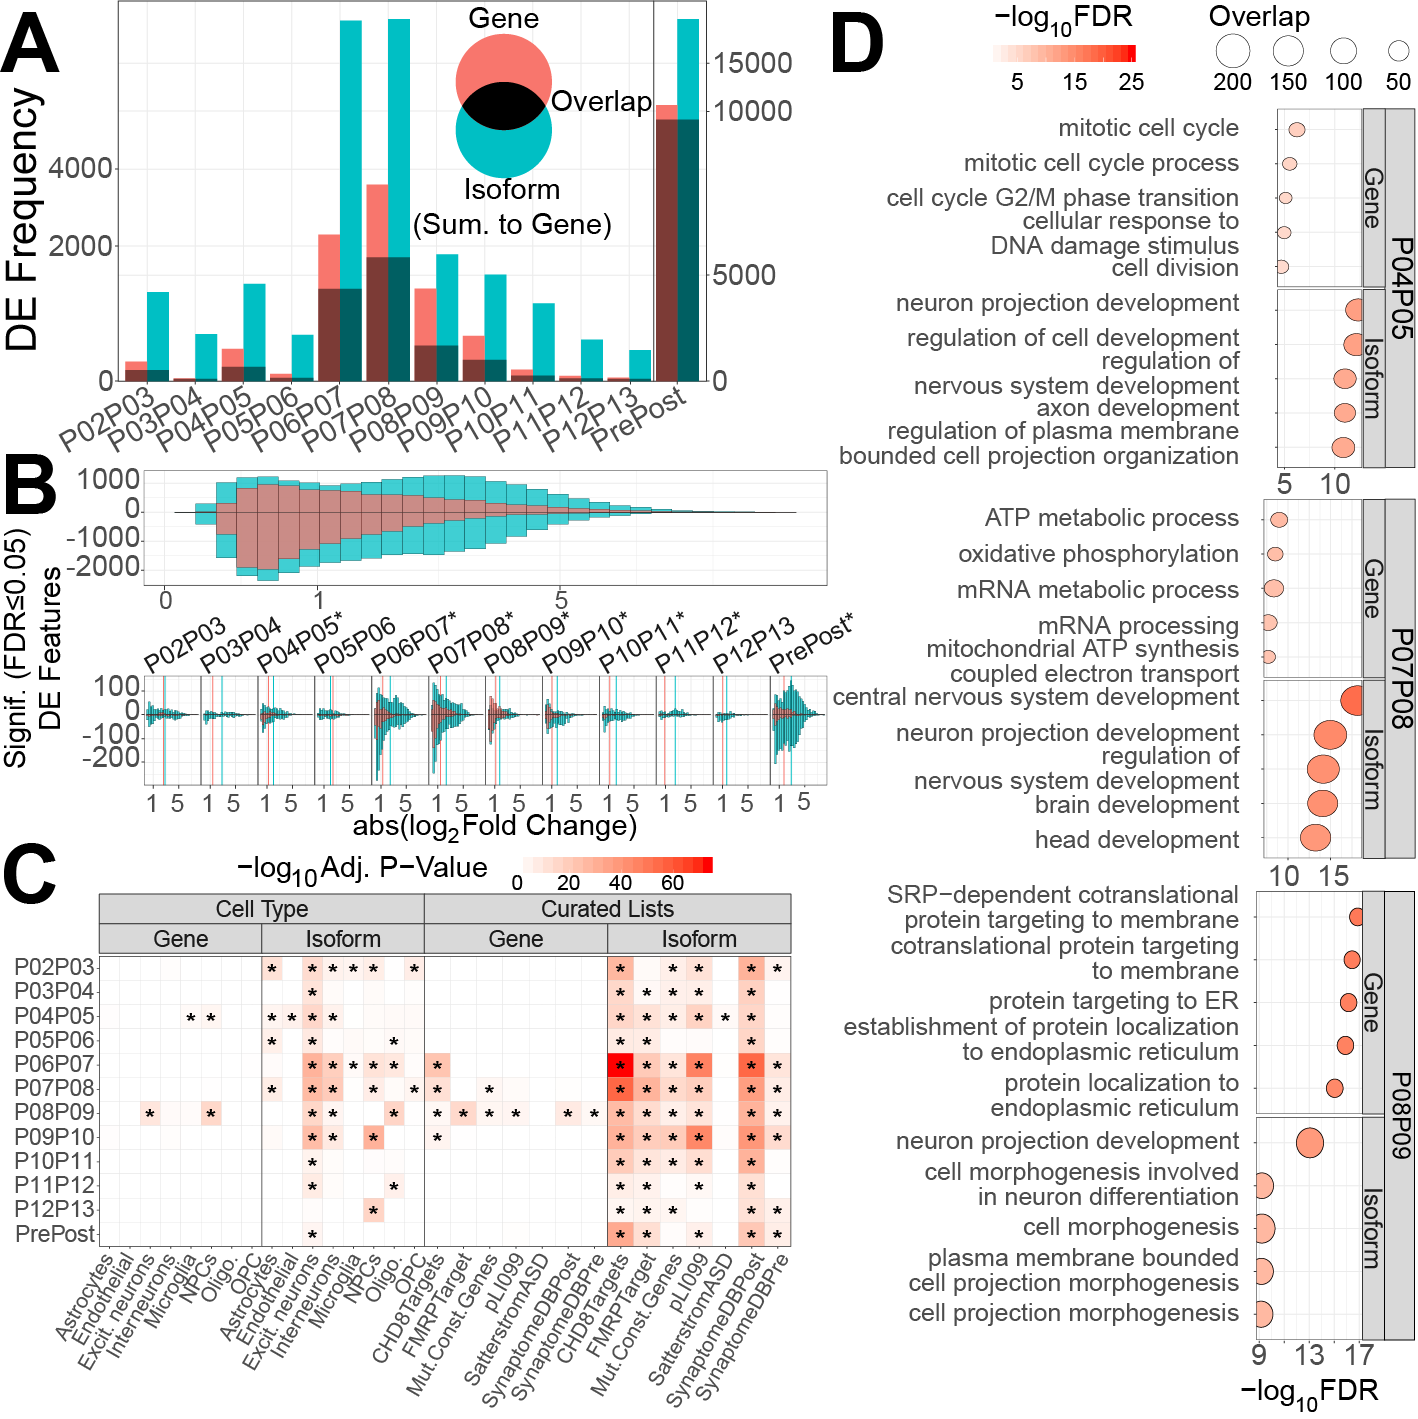
\includegraphics[width=\textwidth]{figure1}
  \caption[Differential expression analysis of gene and isoform quantification data.]
{Differential expression analysis of gene and isoform quantification data. A) Frequency of significant differential expression results at gene-level and isoform-level (summarized to distinct gene parents). B) Effect size (absolute log2 fold change) distribution using total DE results (top) or DE per developmental period contrast (bottom). Average absolute effect sizes for gene data and isoform data are marked by colored vertical lines and differences were tested with two-sample T-tests (*FDR < 0.05). C) Fisher-exact test of enrichment of genes differentially expressed specifically using isoform-level quantifications versus genes specifically differentially expressed with gene-level quantifications. D) Functional enrichment analysis of features specifically DE in either dataset from selected comparisons shows higher signals for nervous system related processes specifically in isoform-level analysis and not with gene-level analysis.}
\end{figure}

\begin{figure}[h]
  \centering
  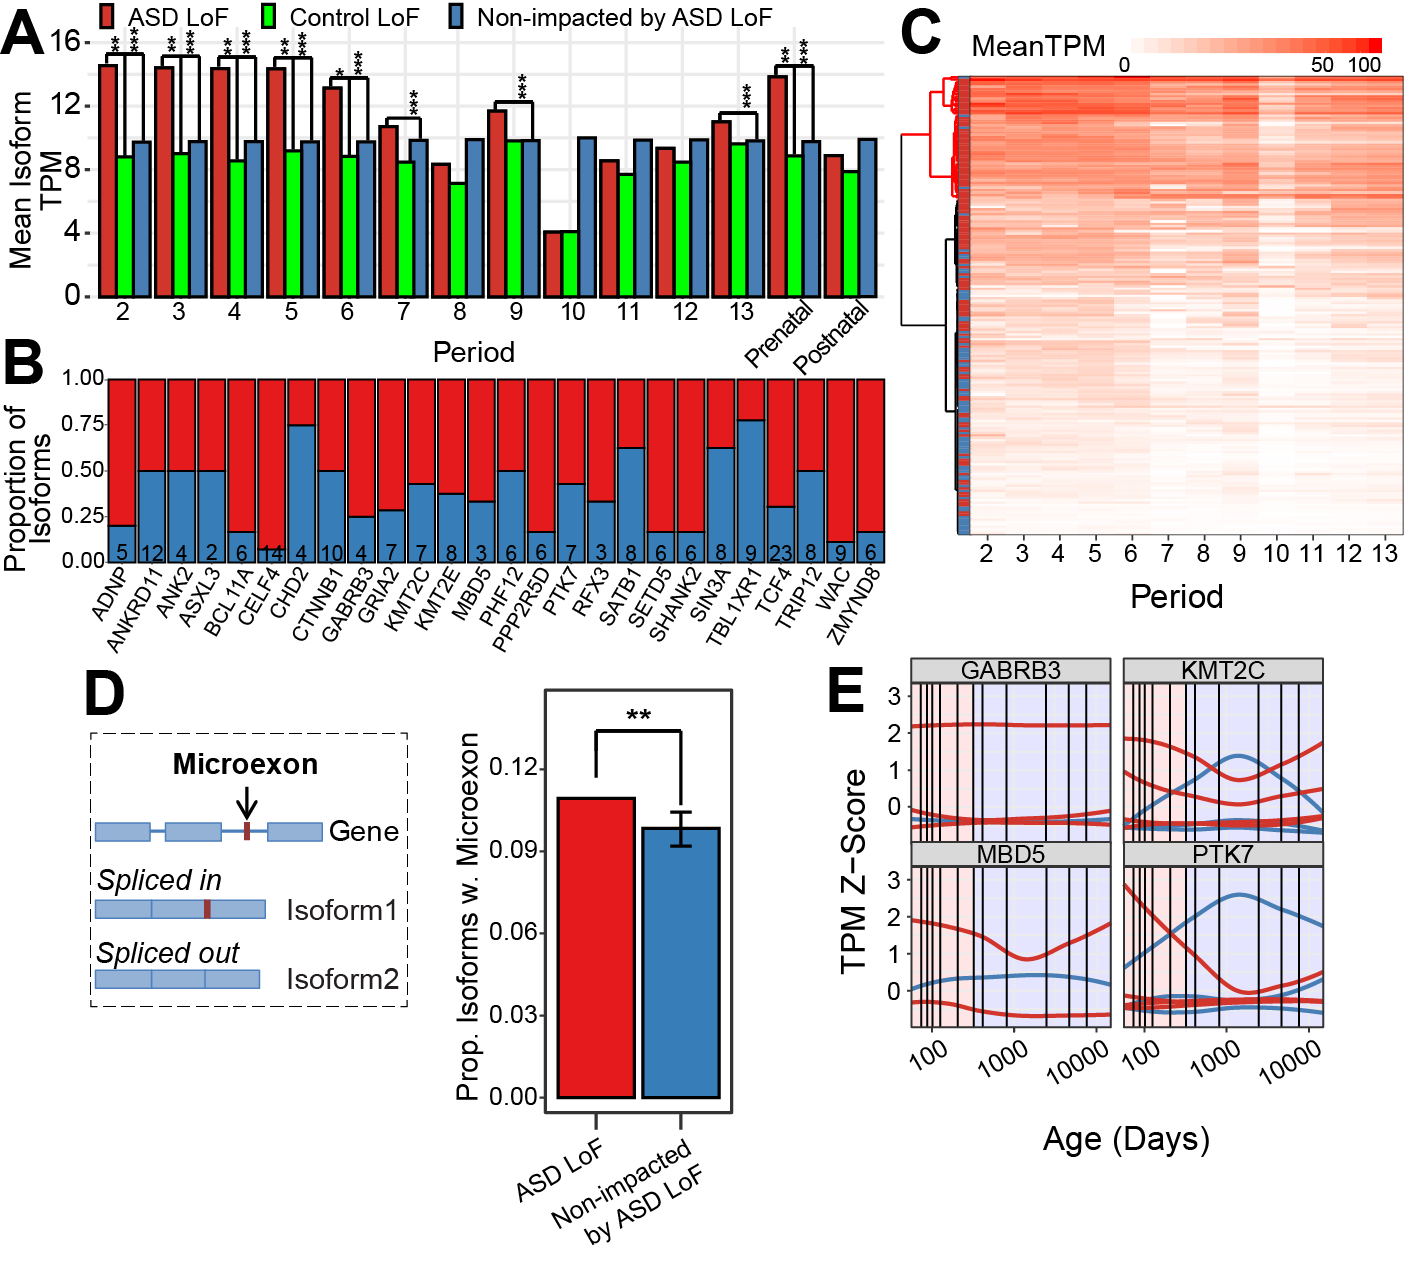
\includegraphics[width=\textwidth]{figure2}
  \caption[Rare de novo ASD loss of function variants.]
{Rare de novo ASD loss of function variants. A) Mean isoform TPM expressions of isoforms impacted by rare de novo ASD LoF variants (ASD LoF) were compared to those of control targets (Control LoF) and non-impacted isoforms (Non-impacted by ASD LoF). B) Proportion of protein-coding isoforms of high-risk ASD genes, specifically differentially expressed at isoform level, either impacted or not impacted by rare de novo ASD LoF variants. C) Ward hierarchical clustering of isoforms from B) and heatmap of average expression per developmental period per isoform. D) Schematic of definition of alternatively regulated microexon (left), along with proportions of isoforms carrying microexons (right), stratified by impact status. E) Selected expression profiles show high variability of sibling isoform expressions transcribed from high-risk ASD genes, and these isoforms tend to be more highly expressed prenatally. $*P \leq 0.1, **P \leq 0.05, ***P \leq 0.01$}
\end{figure}

\begin{figure}[h]
  \centering
  \caption[Gene and isoform co-expression modules reflect distinct signals in neurodevelopment.]
{Gene and isoform co-expression modules reflect distinct signals in neurodevelopment. A) Modules clustered by module eigengene (top); module eigengene-developmental period associations measured by linear mixed effect model beta coefficients (middle); Fisher-exact enrichment tests against cell-type and literature-curated gene lists (bottom). B) Module eigengene expression profiles of modules most significantly associated with each cell type: Astrocytes, iM25; Oligodendrocytes, iM6; Microglia, iM36; NPCs, iM10; Excitatory neurons, iM2; Interneurons, iM17. C) Normalized module impact rate, per module and per status. Modules were selected based on significantly higher impact rate by ASD cases as compared to controls (permutation test, 1000 permutations, FDR $\leq$ 0.05). D) Functional enrichment for significantly impacted modules shows overrepresentation of processes related to DNA metabolic processes, RNA splicing, synapse structure and synapse organization. E) Gene-level PPIs overlaid onto gM1 and iM1, after filtering for direct connections between ASD risk features and ASD LoF features and retaining edges in the top 10\% of Pearson correlation coefficients; both ASD LoF and Non-impacted by ASD LoF isoforms are shown for ASD risk genes, whereas only ASD LoF isoforms are shown for non-risk genes. Module iM1 shows differential connectivity strengths among sibling isoforms, and impacted isoforms show higher PCCs through gene-level PPIs relative to unaffected sibling isoforms. ASD risk genes with differentially impacted isoforms are highlighted in turquoise.}
\end{figure}
\begin{figure}[h]
  \centering
  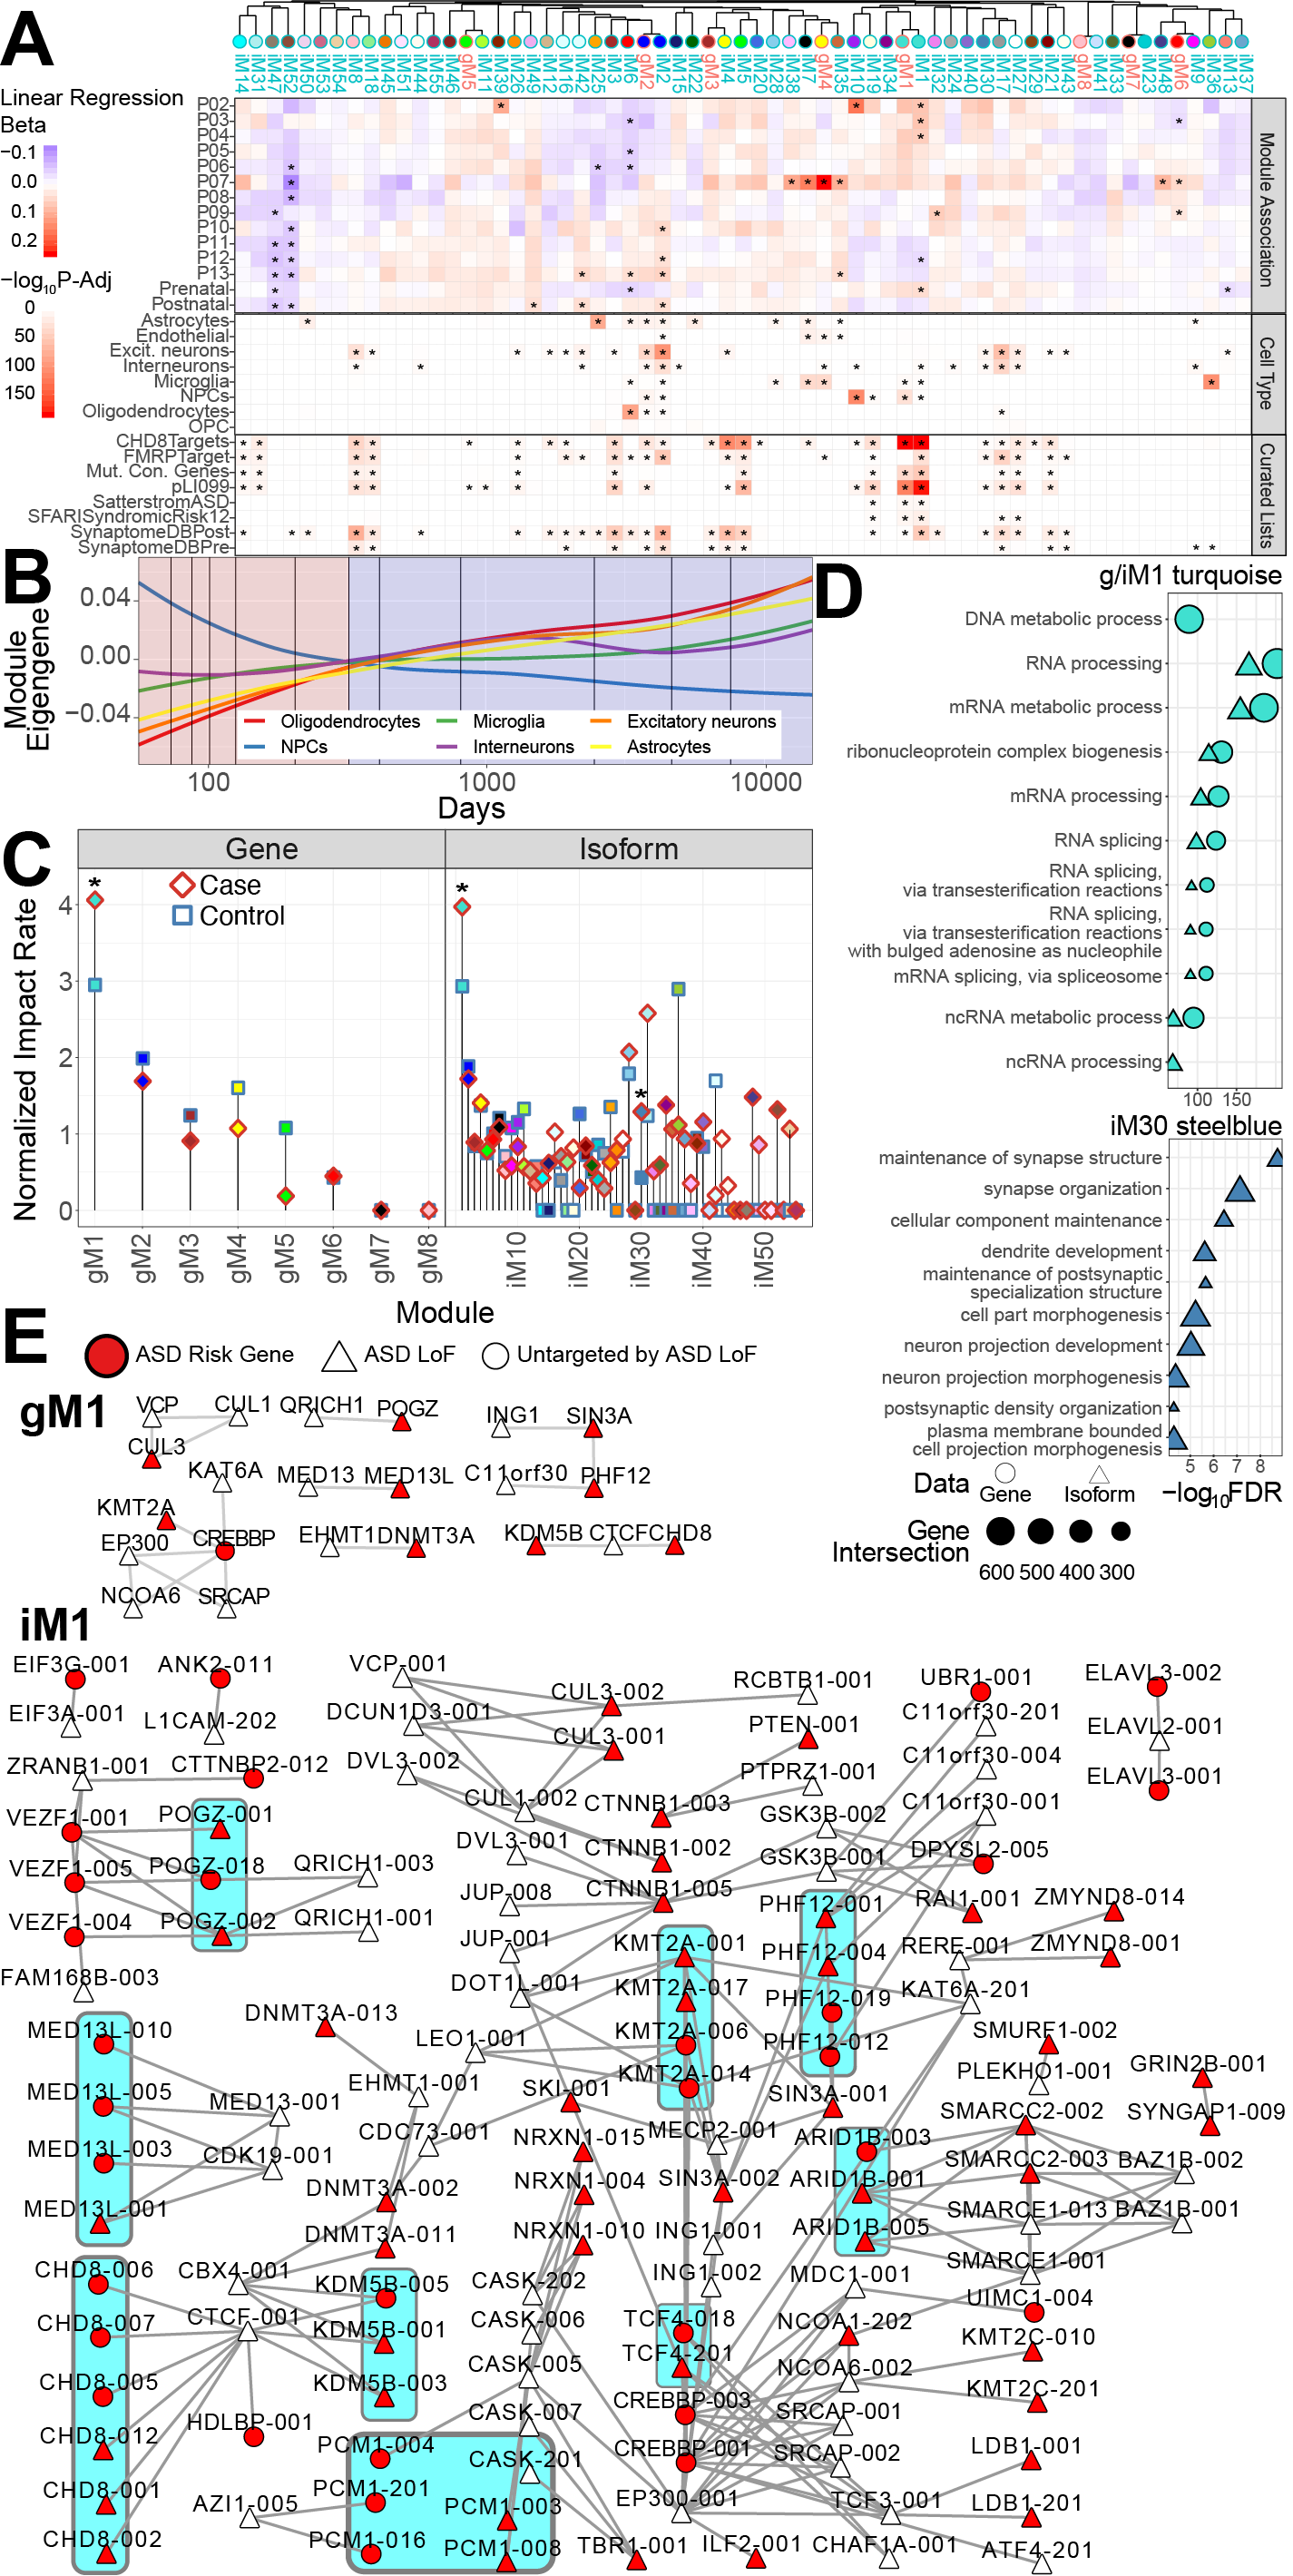
\includegraphics[width=0.65\textwidth]{figure3}
\end{figure}

\begin{figure}[h]
  \centering
  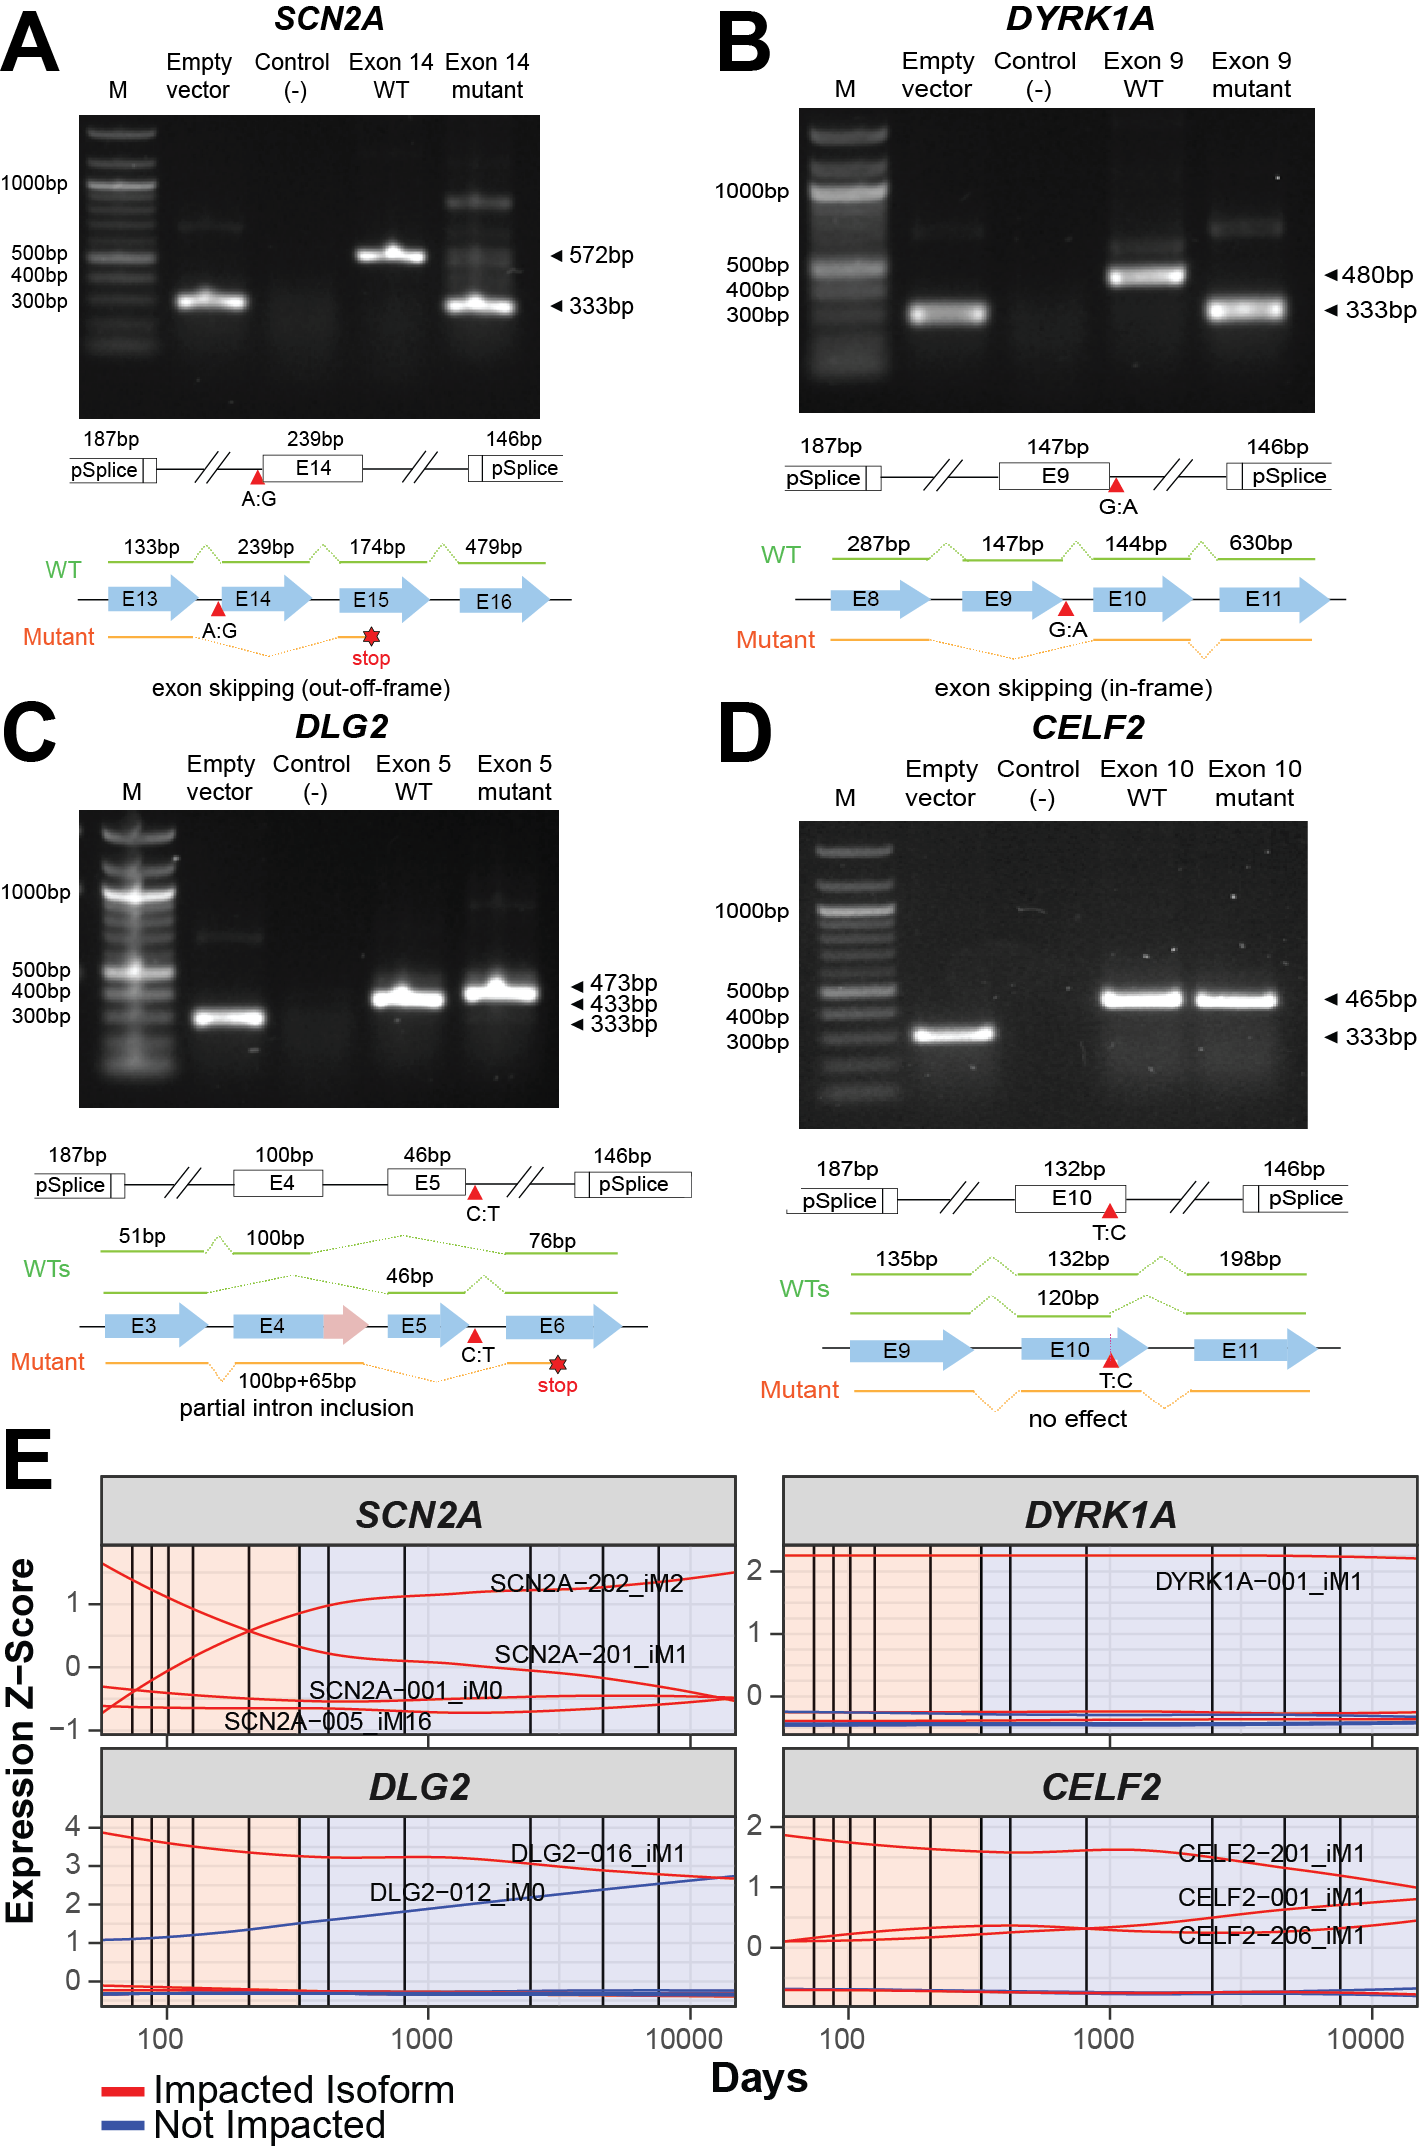
\includegraphics[width=0.75\textwidth]{figure4}
  \caption[Gene and isoform co-expression modules reflect distinct signals in neurodevelopment.]
{Functional effect of the de novo splice site mutations from the patients with neurodevelopmental diseases. Minigene assays demonstrate the effect of splice site mutations in four genes. (A) \textit{SCN2A}; (B) \textit{DYRK1A}; (C) \textit{DLG2}; and (D) \textit{CELF2}. Schematic representation of the cloned minigenes, the expected splicing patterns, and the impact of the mutations are shown below the gel image. Numbers denote base pairs; M: molecular marker; E: exon. E) Expression profiles of the brain-expressed isoforms transcribed by these four genes, annotated with module memberships; highly overlapping expression profiles are unlabeled for readability.}
\end{figure}

\begin{figure}[h]
  \centering
  \caption[The de novo autism splice site mutation causes exon skipping in \textit{BTRC} isoforms and reduces their translational efficiency.]
{The de novo autism splice site mutation causes exon skipping in \textit{BTRC} isoforms and reduces their translational efficiency. A) The exon structure of three splicing isoforms of the \textit{BTRC} gene showing positions of the cloned abridged introns and the splice site mutation; numbers denote base pairs; B) Minigene assays demonstrate exon 4 skipping as a result of the splice site mutation. The assays show the RT-PCR results performed using total RNA from HeLa cells transfected with \textit{BTRC} minigene constructs; numbers denote base pairs; C) Splicing assays with the full-length constructs carrying abridged introns confirm exon skipping observed in the minigene assays; D) Immunoblotting (IB) from the whole cell lysates of HeLa cells transfected with different \textit{BTRC} minigene constructs and an empty vector, as indicated. Membranes were probed to observe \textit{BTRC} overexpression, and to investigate expression of p-$\beta$-catenin, \textit{Cul1} and \textit{SKP1}. $\beta$-actin was used as loading control. Immunoprecipitation was performed with the antibody recognizing V5-tag and proteins were detected by IB with the p-$\beta$-catenin, \textit{Cul1}, \textit{SKP1} and V5 antibodies. The splice site mutation causes reduced translational efficiency of both BTRC\_1Mut and BTRC\_1Mut mutant isoforms as compared to their wild type counterparts; E) Quantification of protein pull-downs with V5-IP using ImageJ software. The band intensity values were normalized to WT expression levels. Error bars represent 95$\%$ confidence intervals (CI) based on 3 independent experiments. On average, 40$\%$ reduction of \textit{BTRC} protein expression is observed as a result of a mutation. Consequently, the reduction of the corresponding \textit{BTRC} binding partners (p-$\beta$-catenin, \textit{Cul1}, and \textit{SKP1}) is also observed. F) Expression profiles of brain-expressed \textit{BTRC} isoforms show higher expression of ASD-impacted \textit{BTRC}-001 and \textit{BTRC}-002. Numbers denote base pairs (A, B, C) or kDa (D). $*P \leq 0.05, **P \leq 0.01, ***P \leq 0.001$.}
\end{figure}
\begin{figure}[h]
  \centering
  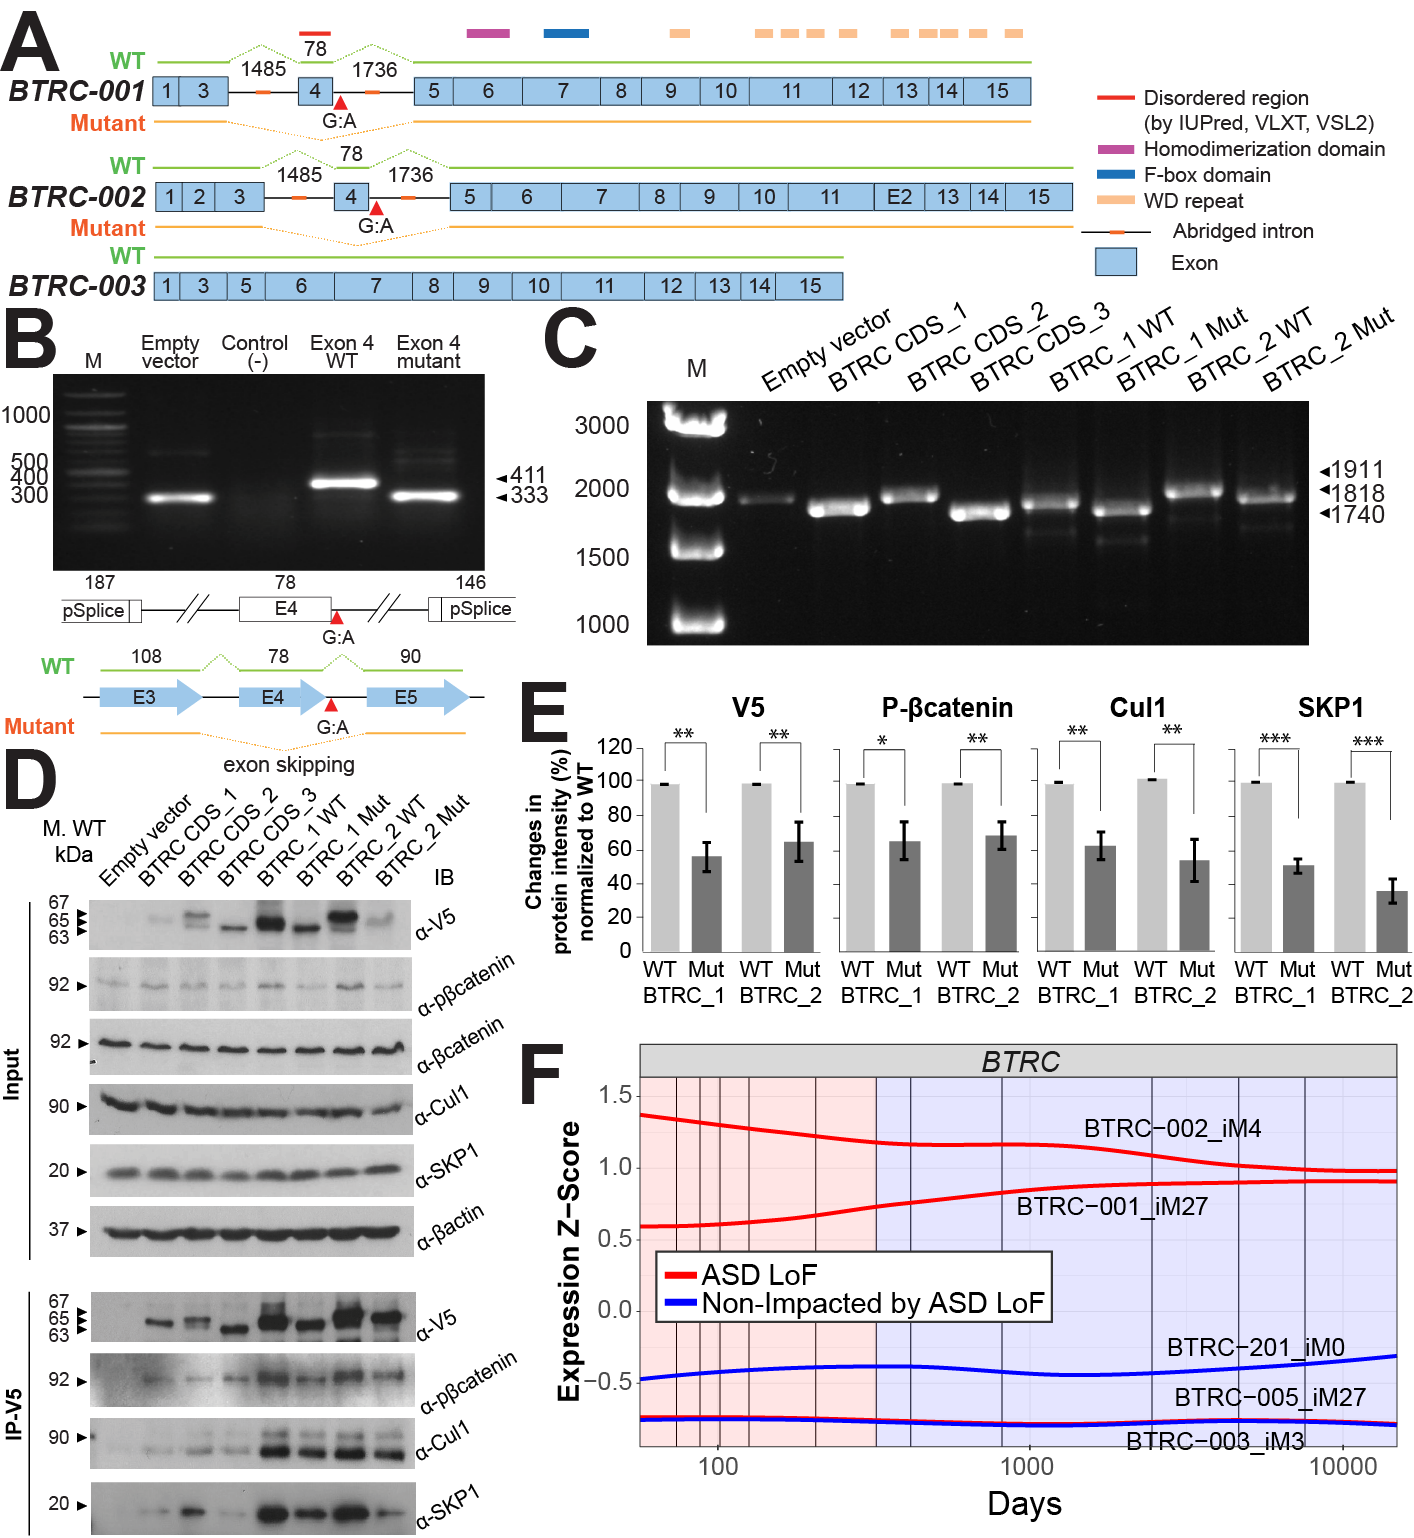
\includegraphics[width=\textwidth]{figure5}
\end{figure}

\chapter{Supplementary Figures}
\clearpage

\begin{suppfigure}[h]
  \centering
  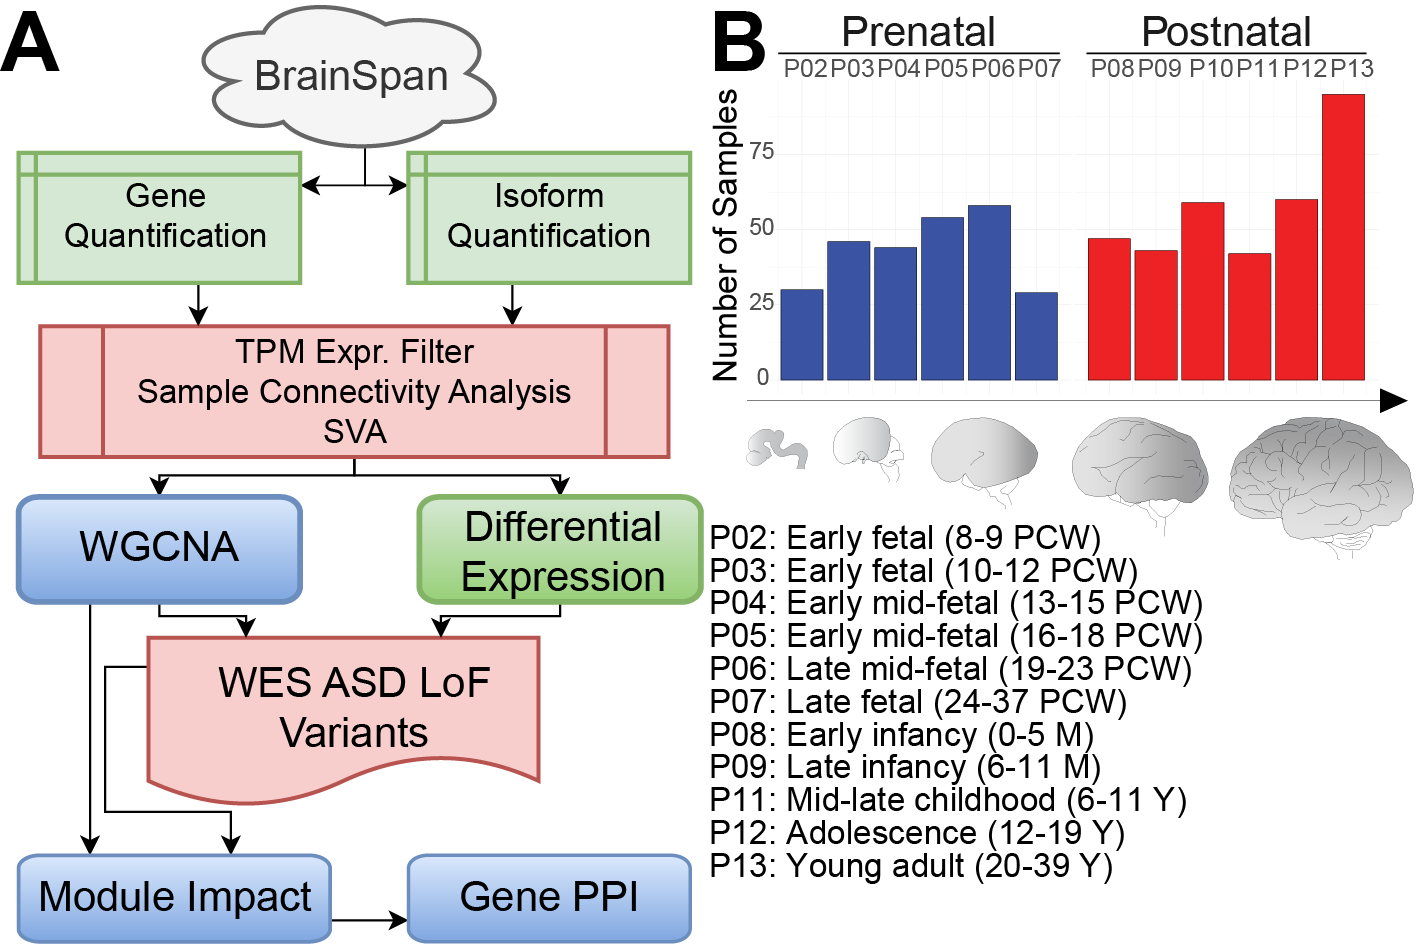
\includegraphics[width=1\textwidth]{suppfigure1}
  \caption[RNA-Seq data was obtained from BrainSpan.]
{RNA-Seq data was obtained from BrainSpan. A) Schematic of bioinformatics analysis of BrainSpan data: Beginning with gene and isoform quantifications downloaded from BrainSpan, features were filtered based on TPM. Outlier samples were detected and removed. Surrogate Variable Analysis was performed to account for latent batch effects. Temporal differential expression was performed on both datasets. WGCNA co-expression networks were created and analyzed on both datasets. Whole exome sequencing data was filtered for LoF variants and mapped to features. B) Initial samples were divided into distinct developmental periods.}
\end{suppfigure}

\begin{suppfigure}[h]
  \centering
  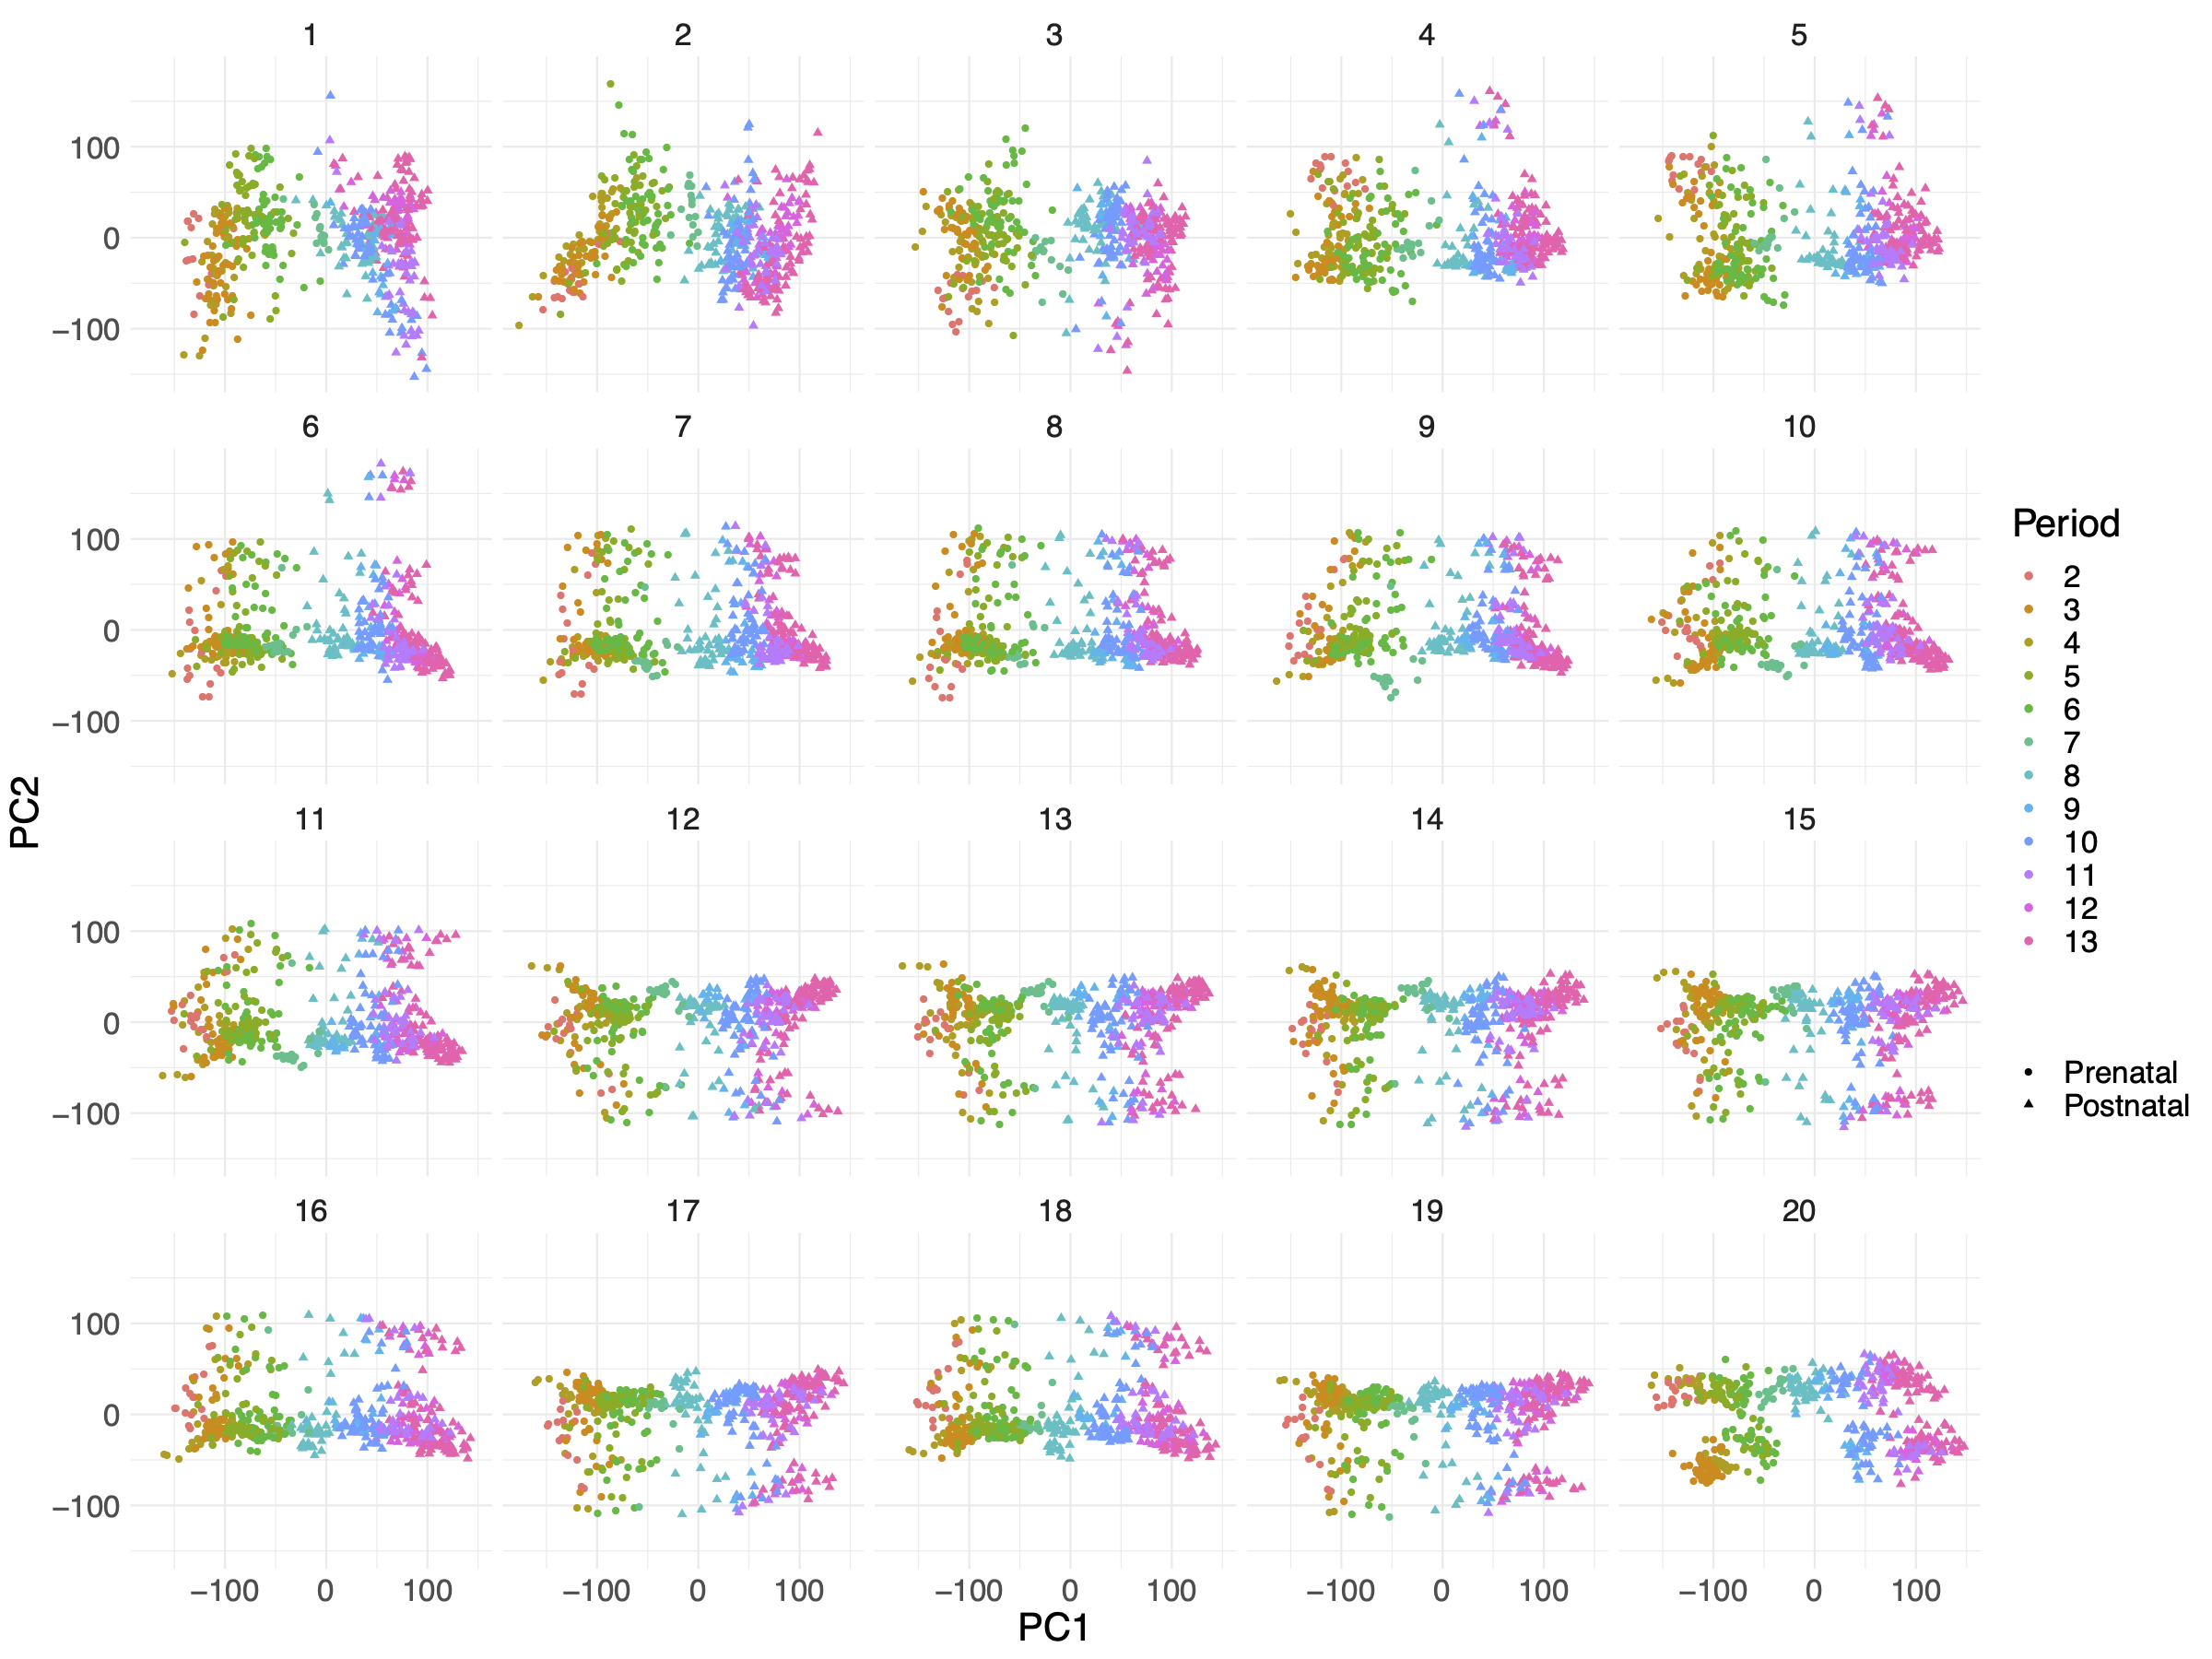
\includegraphics[width=1\textwidth]{suppfigure2}
  \caption[Principal components analysis of transformed gene quantifications.]
{Principal components analysis of transformed gene quantifications. Gene expression data was transformed through regression of relevant covariates (age, brain region, gender, ethnicity, study site, surrogate variables) for each count of surrogate variables analyzed to determine the appropriate number of surrogate variables.}
\end{suppfigure}

\begin{suppfigure}[h]
  \centering
  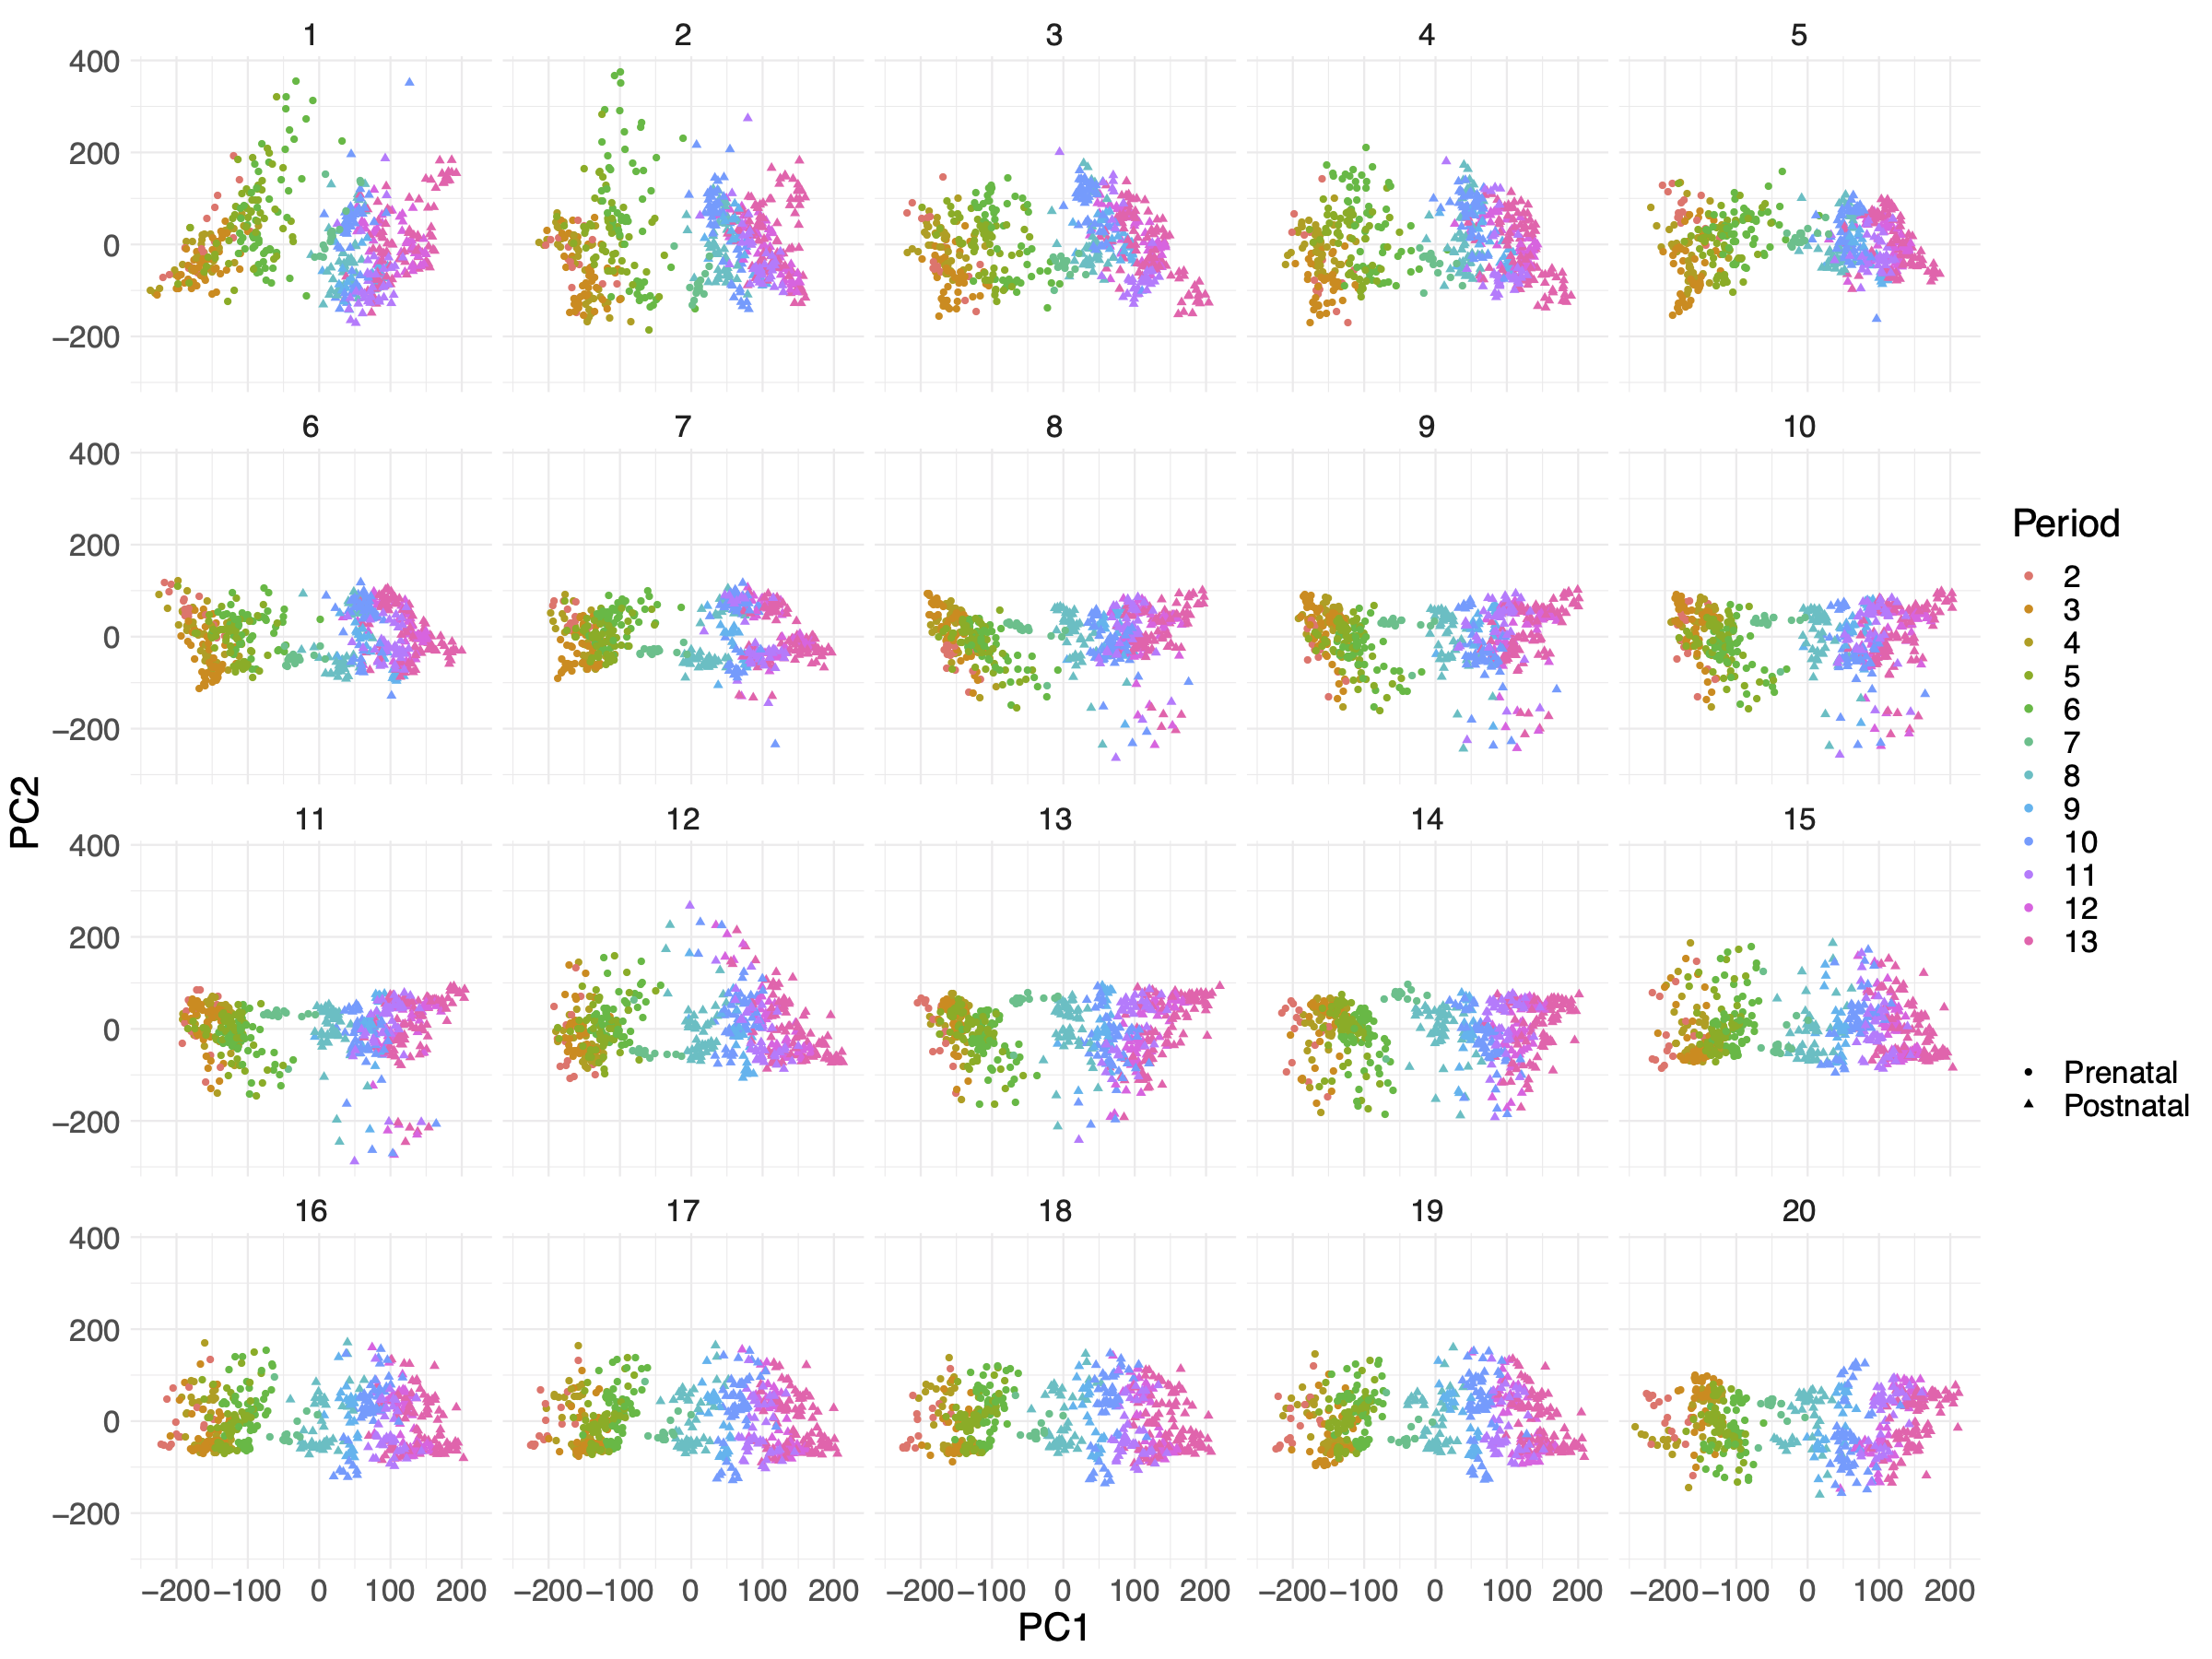
\includegraphics[width=1\textwidth]{suppfigure3}
  \caption[Principal components analysis of transformed isoform quantifications.]
{Principal components analysis of transformed isoform quantifications. Isoform expression data was transformed through regression of relevant covariates (age, brain region, gender, ethnicity, study site, surrogate variables) for each count of surrogate variables analyzed to determine the appropriate number of surrogate variables.}
\end{suppfigure}

\begin{suppfigure}[h]
  \centering
  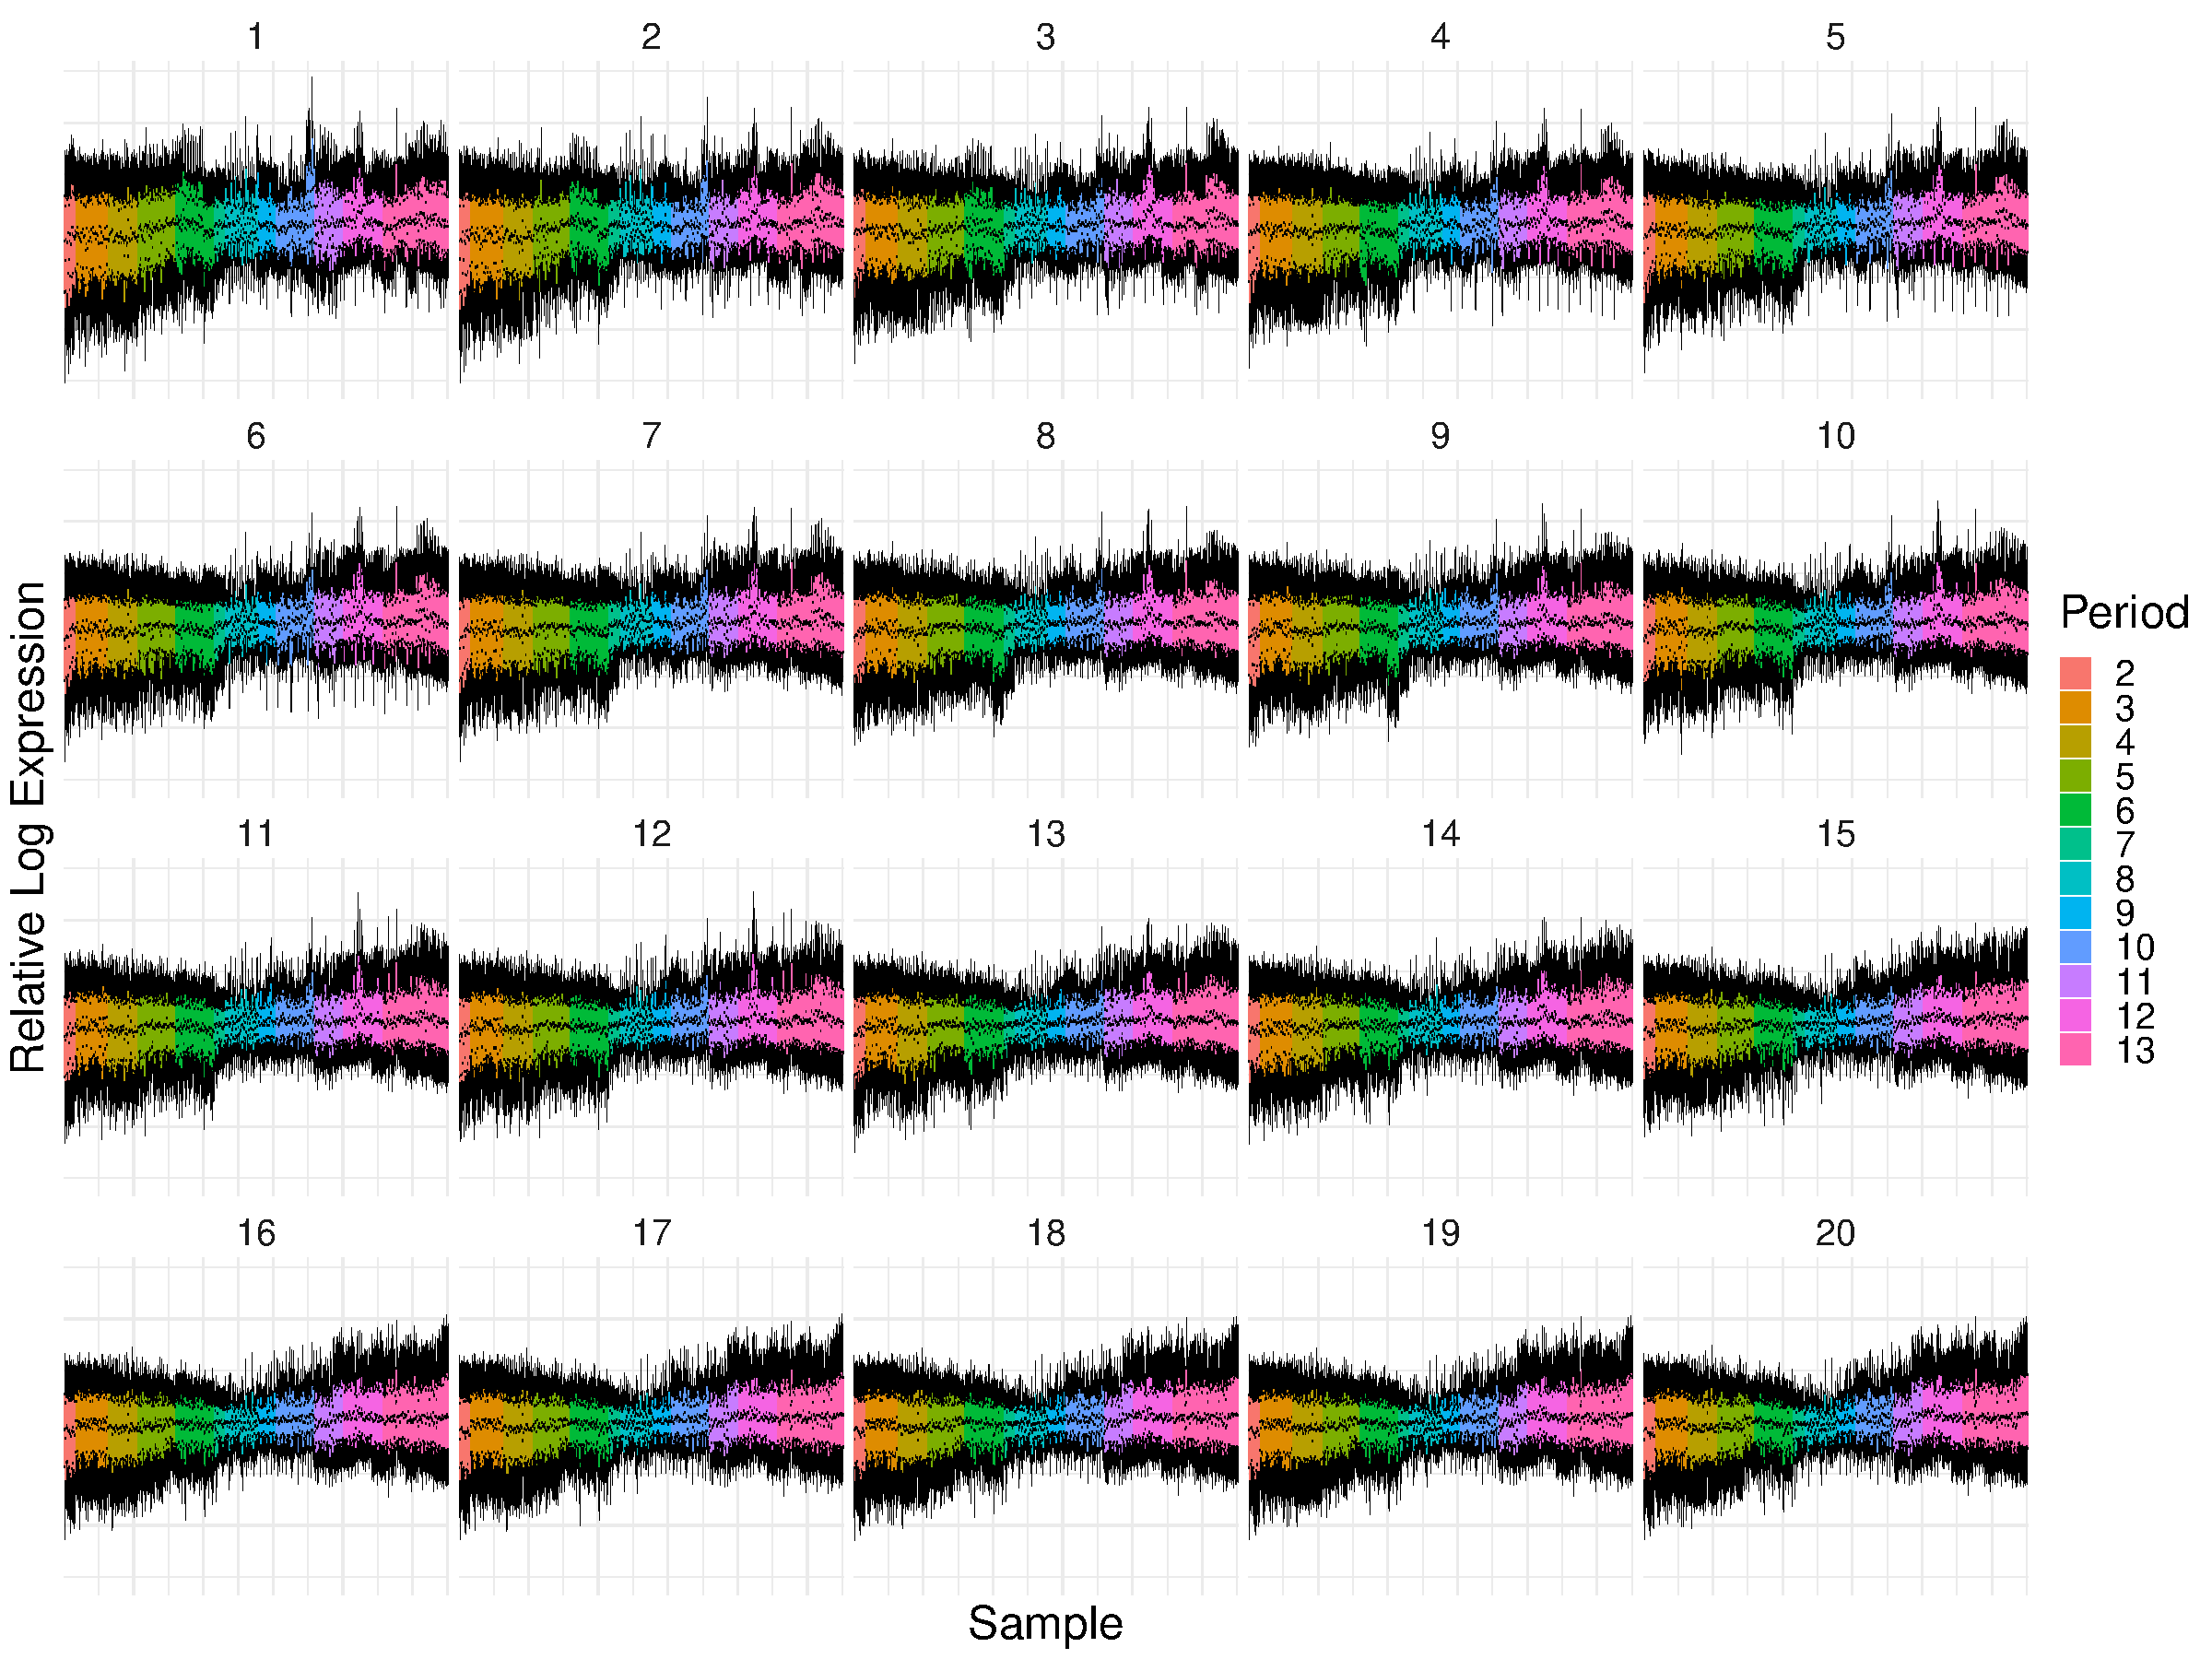
\includegraphics[width=1\textwidth]{suppfigure4}
  \caption[Relative log expression analysis of transformed gene quantifications.]
{Relative log expression analysis of transformed gene quantifications. Gene relative log expressions were calculated, per sample, to find moment of relative log expression stability in surrogate variable selection.}
\end{suppfigure}

\begin{suppfigure}[h]
  \centering
  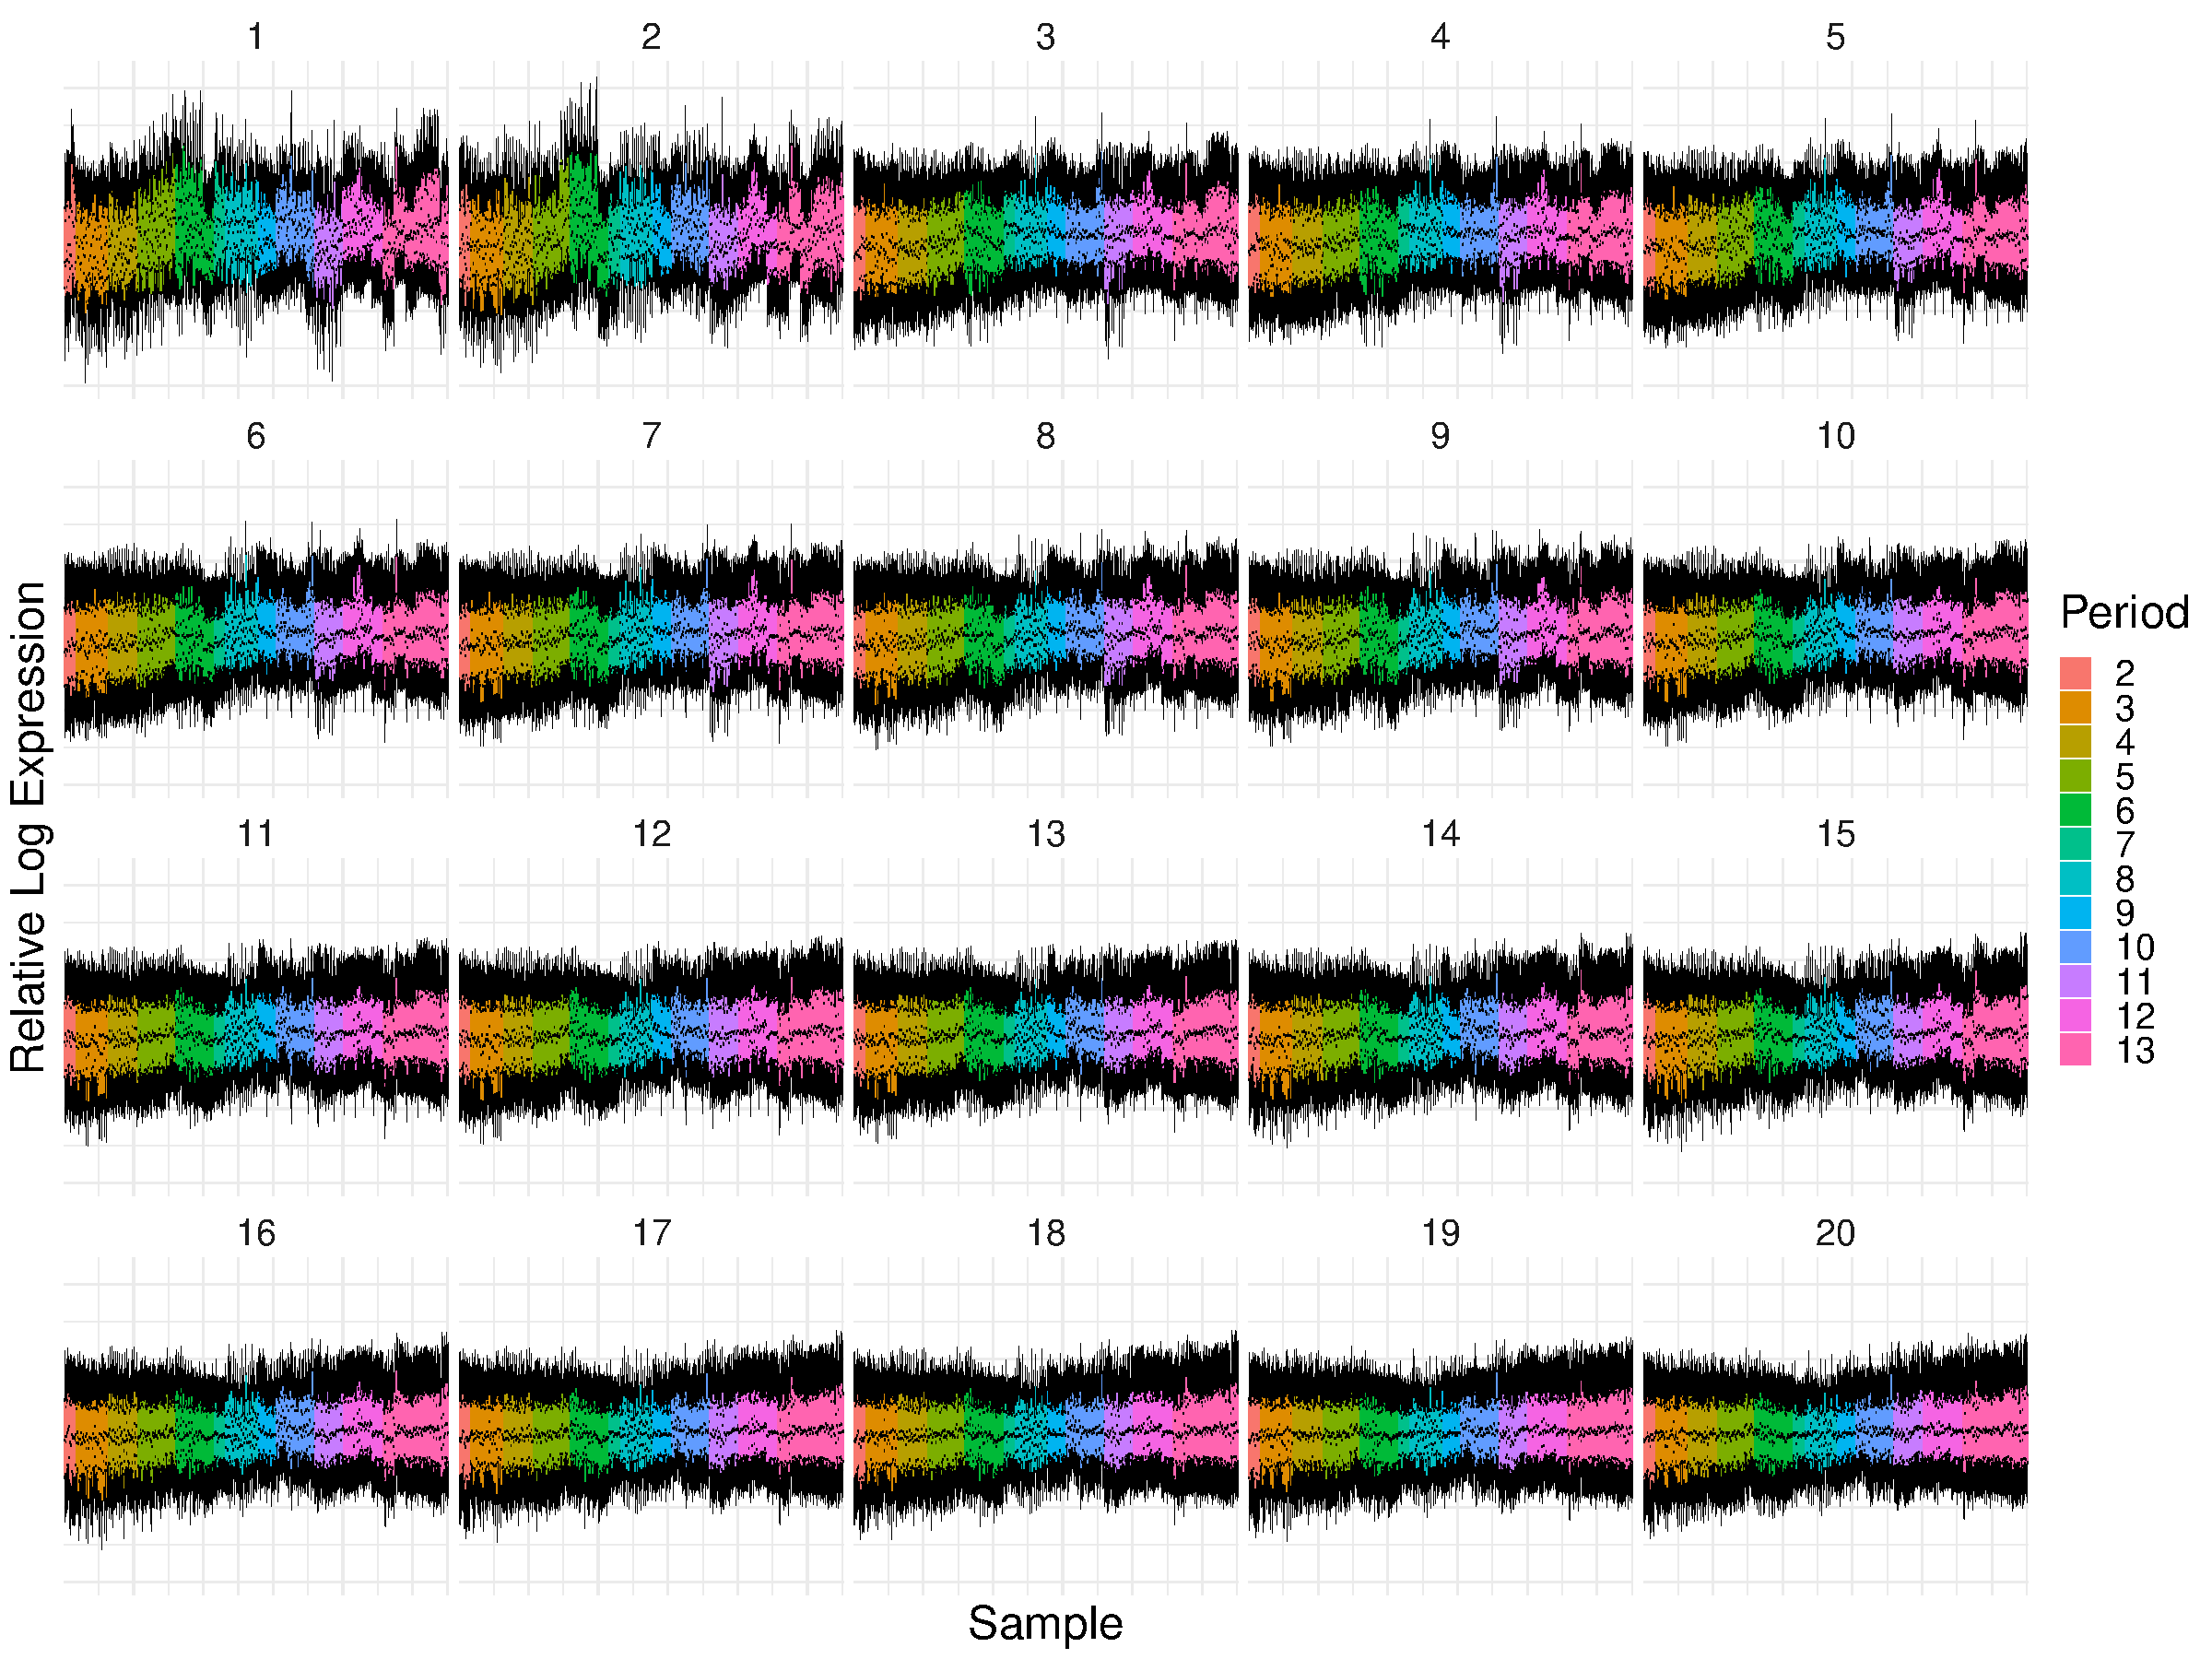
\includegraphics[width=1\textwidth]{suppfigure5}
  \caption[Relative log expression analysis of transformed isoform quantifications.]
{Relative log expression analysis of transformed isoform quantifications. Isoform relative log expressions were calculated, per sample, to find moment of relative log expression stability in surrogate variable selection.}
\end{suppfigure}

\begin{suppfigure}[h]
  \centering
  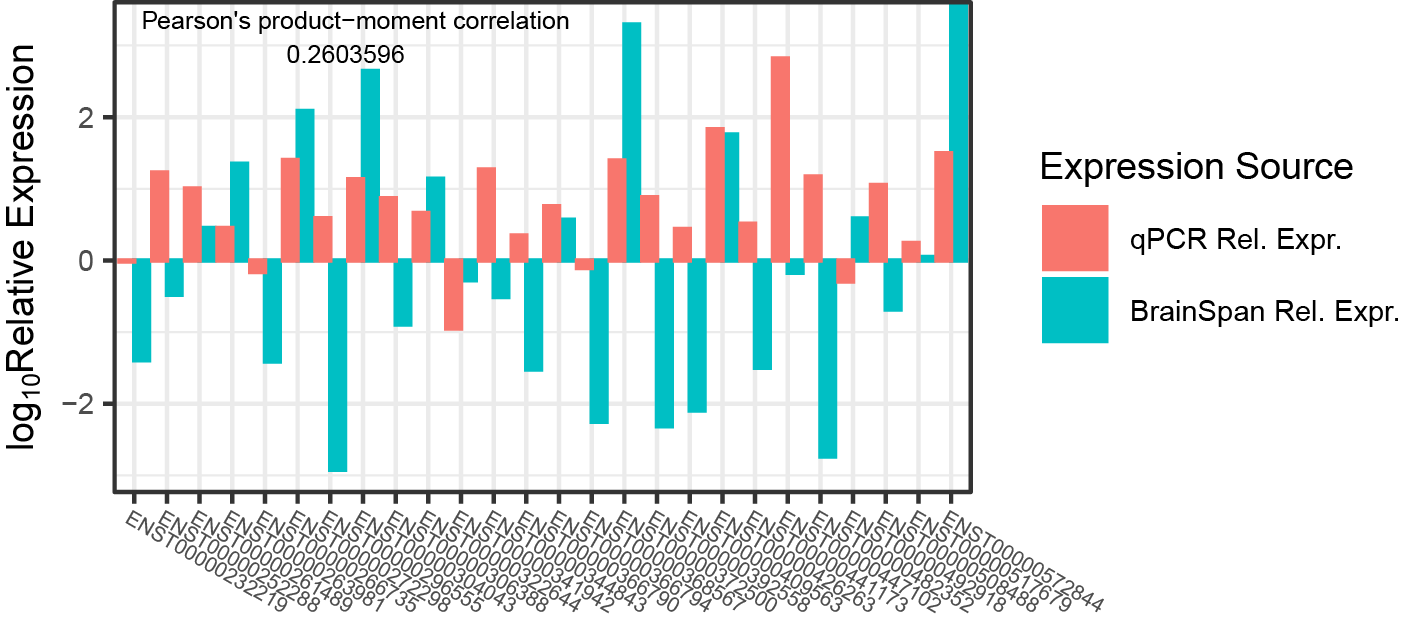
\includegraphics[width=1\textwidth]{suppfigure6}
  \caption[Comparison of relative expression from qPCR and BrainSpan.]
{Comparison of relative expression from qPCR and BrainSpan. Age- and gender-matched samples were compared for the isoforms of 14 genes; positive Pearson correlation was found for the sign of relative expressions.}
\end{suppfigure}
\clearpage
\pagebreak
\newpage
This thesis, in full, is currently being prepared for submission for publication of the material. Chau, Kevin K.; Zhang, Pan; Urresti, Jorge; Amar, Megha; Pramod, Akula Bala; Corominas, Roser; Lin, Guan Ning; Iakoucheva, Lilia M. The thesis author was the primary investigator and author of this material. \par

%% END MATTER
\bibliographystyle{unsrt}
\bibliography{thesis}


\chapter*{Supplementary Files}
\begin{table}[!ht]
\caption[chau\_01\_supplementary\_table\_1.xlsx, This table consists of relevant data for validation of BrainSpan TPM expression values against age-matched qPCR results.]
{This table consists of relevant data for validation of BrainSpan TPM expression values against age-matched qPCR results.}
\begin{tabular}{|p{1in}|p{2in}|p{3in}|}
\end{tabular}
\end{table}
\begin{table}[!ht]
\caption[chau\_02\_supplementary\_table\_2.xlsx, Full gene-level differential expression results.]
{Full gene-level differential expression results.}
\begin{tabular}{|p{1in}|p{2in}|p{3in}|}
\end{tabular}
\end{table}
\begin{table}[!ht]
\caption[chau\_03\_supplementary\_table\_3.xlsx, Full isoform-level differential expression results.]
{Full isoform-level differential expression results.}
\end{table}
\begin{table}[!ht]
\caption[chau\_04\_supplementary\_table\_4.xlsx]
{Composition of differential expression results.}
\end{table}
\begin{table}[!ht]
\caption[chau\_05\_supplementary\_table\_5.xlsx, Gene ontology enrichment analysis results for gene-level differential expression analysis.]
{Gene ontology enrichment analysis results for gene-level differential expression analysis.}
\end{table}
\begin{table}[!ht]
\caption[chau\_06\_supplementary\_table\_6.xlsx, Gene ontology enrichment analysis results for isoform-level differential expression analysis.]
{Gene ontology enrichment analysis results for isoform-level differential expression analysis.}
\end{table}
\begin{table}[!ht]
\caption[chau\_07\_supplementary\_table\_7.xlsx, Compiled and annotated variants table.]
{Compiled and annotated variants table.}
\end{table}
\begin{table}[!ht]
\caption[chau\_08\_supplementary\_table\_8.xlsx, Gene co-expression module assignments.]
{Gene co-expression module assignments.}
\end{table}
\begin{table}[!ht]
\caption[chau\_09\_supplementary\_table\_9.xlsx, Isoform co-expression module assignments.]
{Isoform co-expression module assignments.}
\end{table}
\begin{table}[!ht]
\caption[chau\_10\_supplementary\_table\_10.xlsx, Gene ontology enrichment analysis of gene co-expression modules.]
{Gene ontology enrichment analysis of gene co-expression modules.}
\end{table}
\begin{table}[!ht]
\caption[chau\_11\_supplementary\_table\_11.xlsx, Gene ontology enrichment analysis of isoform co-expression modules]
{Gene ontology enrichment analysis of isoform co-expression modules}
\end{table}
\begin{table}[!ht]
\caption[chau\_12\_supplementary\_table\_12.xlsx, Module impact rate analysis results]
{Module impact rate analysis results}
\end{table}

\end{document}
